\chapter{Model / Experiment Comparison Graphs}
\label{sec:Graphs}

\section{ATF Corridors}

The ATF Corridors experiments consisted of two corridors one on top of the other and connected by a stairwell. The fire, a natural gas sand burner, was located on the first level at the end of the corridor away from the stairwell. The corridor was closed at this end, and open at the same position on the second level. Two-way flow occurred on both levels because make-up air flowed from the opening on the second level down the stairs to the first. The only opening to the enclosure was the open end of the second-level corridor.

Temperatures were measured with seven thermocouple trees. Tree A was located fairly close to the fire on the first level. Tree~B was located halfway down the first-level corridor. Tree~C was close to the stairwell entrance on the first level. Tree~D was located in the doorway of the stairwell on the first level. Tree~E was located roughly along the vertical centerline of the
stairwell. Tree~F was located near the stairwell opening on the second level. Tree~G was located near the exit at the other end of the second-level corridor. The graphs on the following pages show the top and bottom TC from each tree for the given fire sizes of 50~kW, 100~kW, 250~kW, 500~kW, and a mixed HRR ``pulsed'' fire.

HGL temperature and depth reductions were carried out using three arrays of thermocouples in the lower corridor (Trees~A, B, and C) and two arrays in the upper corridor (Trees~G and H).
Ceiling jet temperatures were compared using the top thermocouple in the three downstairs thermocouple trees (Trees~A, B, and C). Since CFAST only computes ceiling jet temperatures in compartments with a fire, no comparisons were made for the upper compartment.

\begin{figure}
\begin{tabular*}{\textwidth}{l@{\extracolsep{\fill}}r}
\includegraphics[width=2.6in]{FIGURES/ATF_Corridors/ATF_Corridors_HGL_Temp_1_050_kW} &
\includegraphics[width=2.6in]{FIGURES/ATF_Corridors/ATF_Corridors_HGL_Height_1_050_kW} \\
\includegraphics[width=2.6in]{FIGURES/ATF_Corridors/ATF_Corridors_HGL_Temp_1_100_kW} &
\includegraphics[width=2.6in]{FIGURES/ATF_Corridors/ATF_Corridors_HGL_Height_1_100_kW} \\
\includegraphics[width=2.6in]{FIGURES/ATF_Corridors/ATF_Corridors_HGL_Temp_1_240_kW} &
\includegraphics[width=2.6in]{FIGURES/ATF_Corridors/ATF_Corridors_HGL_Height_1_240_kW}
\end{tabular*}
\end{figure}

\begin{figure}
\begin{tabular*}{\textwidth}{l@{\extracolsep{\fill}}r}
\includegraphics[width=2.6in]{FIGURES/ATF_Corridors/ATF_Corridors_HGL_Temp_1_250_kW} &
\includegraphics[width=2.6in]{FIGURES/ATF_Corridors/ATF_Corridors_HGL_Height_1_250_kW} \\
\includegraphics[width=2.6in]{FIGURES/ATF_Corridors/ATF_Corridors_HGL_Temp_1_500_kW} &
\includegraphics[width=2.6in]{FIGURES/ATF_Corridors/ATF_Corridors_HGL_Height_1_500_kW} \\
\includegraphics[width=2.6in]{FIGURES/ATF_Corridors/ATF_Corridors_HGL_Temp_1_Mix_kW} &
\includegraphics[width=2.6in]{FIGURES/ATF_Corridors/ATF_Corridors_HGL_Height_1_Mix_kW}
\end{tabular*}
\end{figure}

\begin{figure}
\begin{tabular*}{\textwidth}{l@{\extracolsep{\fill}}r}
\includegraphics[width=2.6in]{FIGURES/ATF_Corridors/ATF_Corridors_HGL_Temp_2_050_kW} &
\includegraphics[width=2.6in]{FIGURES/ATF_Corridors/ATF_Corridors_HGL_Height_2_050_kW} \\
\includegraphics[width=2.6in]{FIGURES/ATF_Corridors/ATF_Corridors_HGL_Temp_2_100_kW} &
\includegraphics[width=2.6in]{FIGURES/ATF_Corridors/ATF_Corridors_HGL_Height_2_100_kW} \\
\includegraphics[width=2.6in]{FIGURES/ATF_Corridors/ATF_Corridors_HGL_Temp_2_240_kW} &
\includegraphics[width=2.6in]{FIGURES/ATF_Corridors/ATF_Corridors_HGL_Height_2_240_kW}
\end{tabular*}
\end{figure}

\begin{figure}
\begin{tabular*}{\textwidth}{l@{\extracolsep{\fill}}r}
\includegraphics[width=2.6in]{FIGURES/ATF_Corridors/ATF_Corridors_HGL_Temp_2_250_kW} &
\includegraphics[width=2.6in]{FIGURES/ATF_Corridors/ATF_Corridors_HGL_Height_2_250_kW} \\
\includegraphics[width=2.6in]{FIGURES/ATF_Corridors/ATF_Corridors_HGL_Temp_2_500_kW} &
\includegraphics[width=2.6in]{FIGURES/ATF_Corridors/ATF_Corridors_HGL_Height_2_500_kW} \\
\includegraphics[width=2.6in]{FIGURES/ATF_Corridors/ATF_Corridors_HGL_Temp_2_Mix_kW} &
\includegraphics[width=2.6in]{FIGURES/ATF_Corridors/ATF_Corridors_HGL_Height_2_Mix_kW}
\end{tabular*}
\end{figure}

\begin{figure}
\begin{tabular*}{\textwidth}{l@{\extracolsep{\fill}}r}
\includegraphics[width=2.6in]{FIGURES/ATF_Corridors/ATF_Corridors_Jet_Temp_050_kW} &
\includegraphics[width=2.6in]{FIGURES/ATF_Corridors/ATF_Corridors_Jet_Temp_100_kW} \\
\includegraphics[width=2.6in]{FIGURES/ATF_Corridors/ATF_Corridors_Jet_Temp_240_kW} &
\includegraphics[width=2.6in]{FIGURES/ATF_Corridors/ATF_Corridors_Jet_Temp_250_kW} \\
\includegraphics[width=2.6in]{FIGURES/ATF_Corridors/ATF_Corridors_Jet_Temp_500_kW} &
\includegraphics[width=2.6in]{FIGURES/ATF_Corridors/ATF_Corridors_Jet_Temp_Mix_kW}
\end{tabular*}
\end{figure}

\clearpage

\section{FM Four Room Including Corridor Test Series}

This data set describes a series of tests conducted in a multiple room configuration with more complex gas burner fires than the previous data set.  This study \cite{Heskestad:1986} was included because, in many ways, it is similar to the smoke movement study performed at NBS \cite{Peacock:1988}, and permits comparisons between two different laboratories. In addition, it expands upon that data set by providing larger a time-varying gas burner fires in a room-corridor configuration. Fire size was about up to 1 MW with a total volume of 200 m$^3$. This study was performed to collect data allowing for variations in fire source, ventilation, and geometry in a multi-compartment structure, especially for situations with closed doors.

\begin{figure}[p]
\begin{tabular*}{\textwidth}{l@{\extracolsep{\fill}}r}
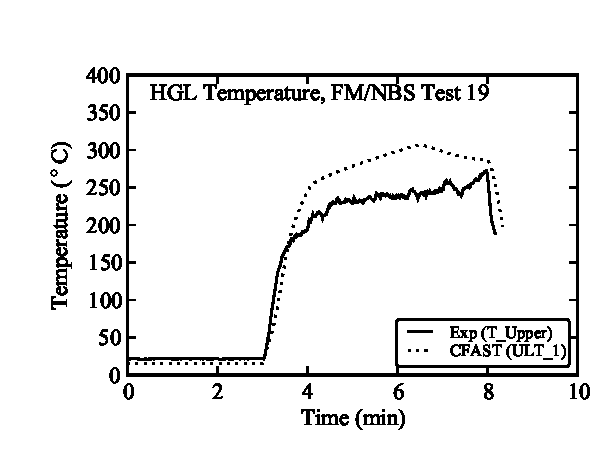
\includegraphics[width=2.6in]{FIGURES/FM_NBS/FM19_1_HGL_Temp} &
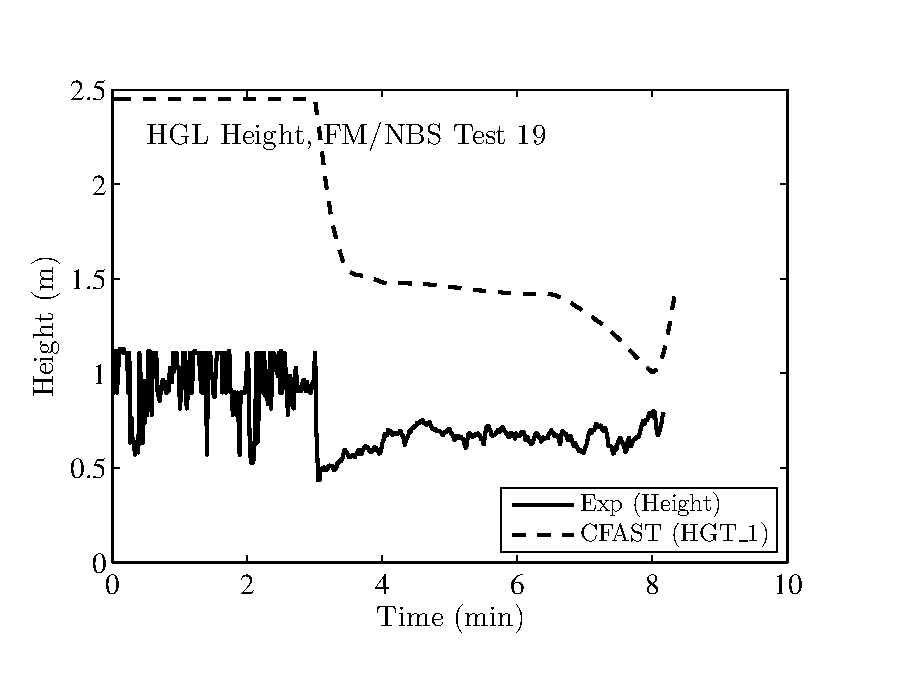
\includegraphics[width=2.6in]{FIGURES/FM_NBS/FM19_1_HGL_Height} \\
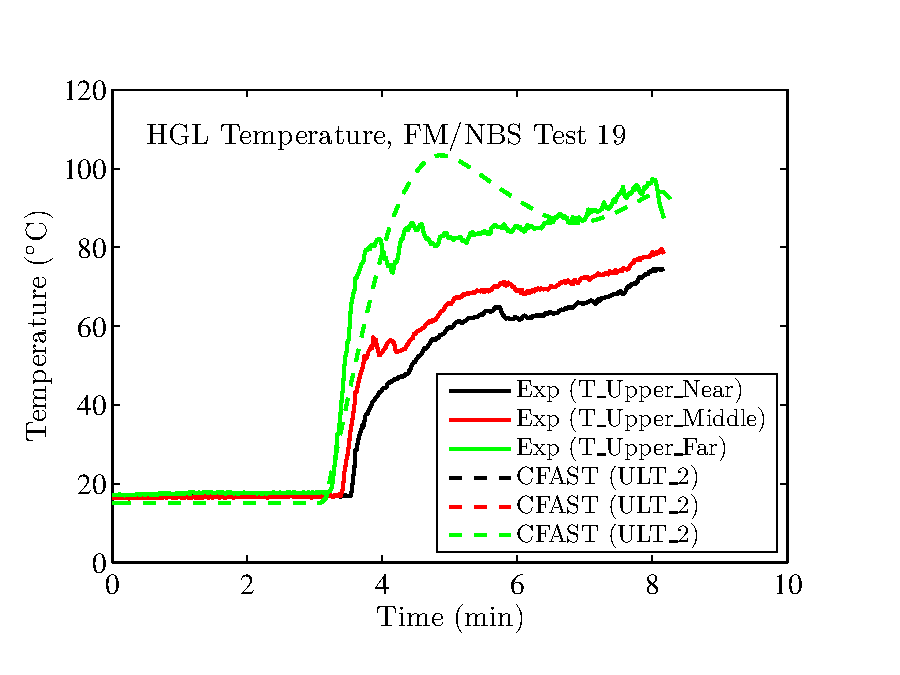
\includegraphics[width=2.6in]{FIGURES/FM_NBS/FM19_2_HGL_Temp} &
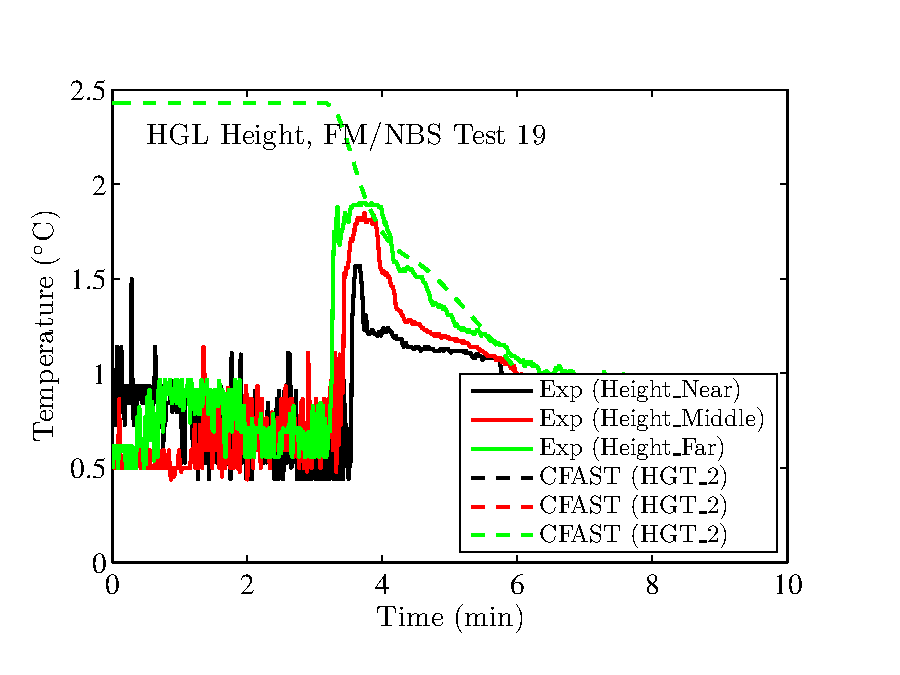
\includegraphics[width=2.6in]{FIGURES/FM_NBS/FM19_2_HGL_Height} \\
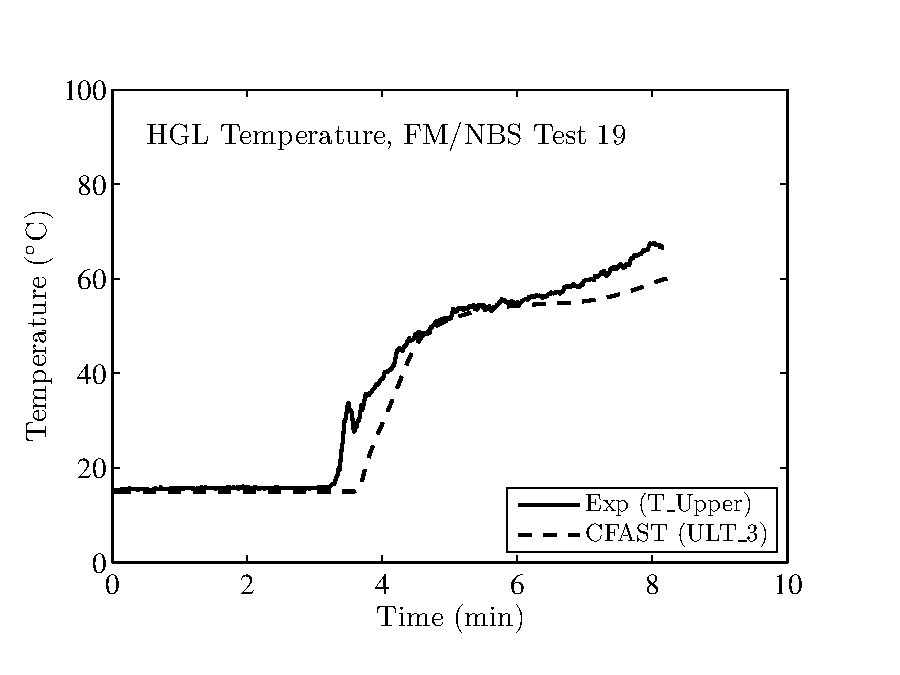
\includegraphics[width=2.6in]{FIGURES/FM_NBS/FM19_3_HGL_Temp} &
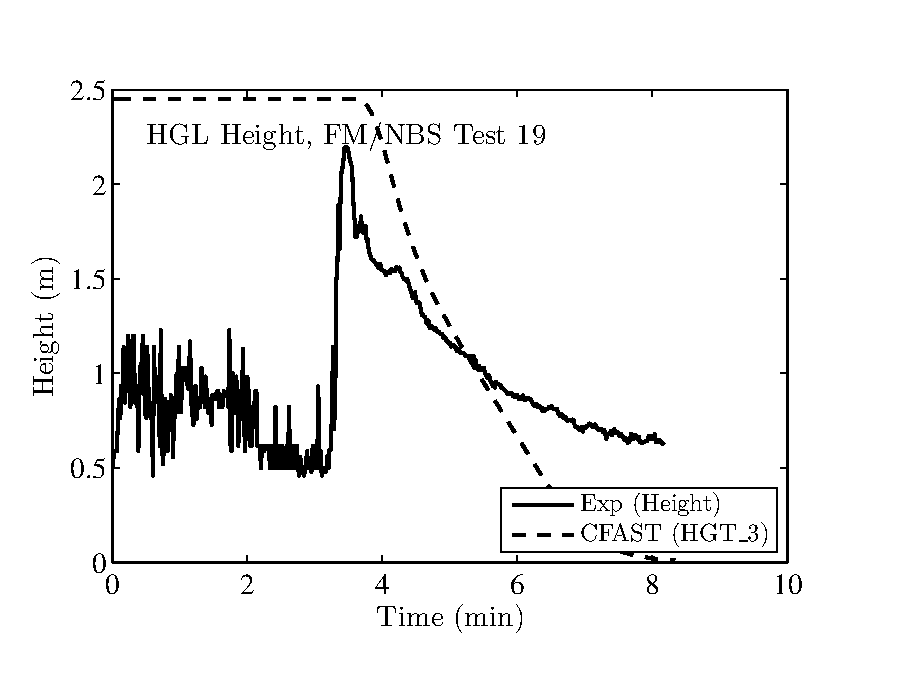
\includegraphics[width=2.6in]{FIGURES/FM_NBS/FM19_3_HGL_Height} \\
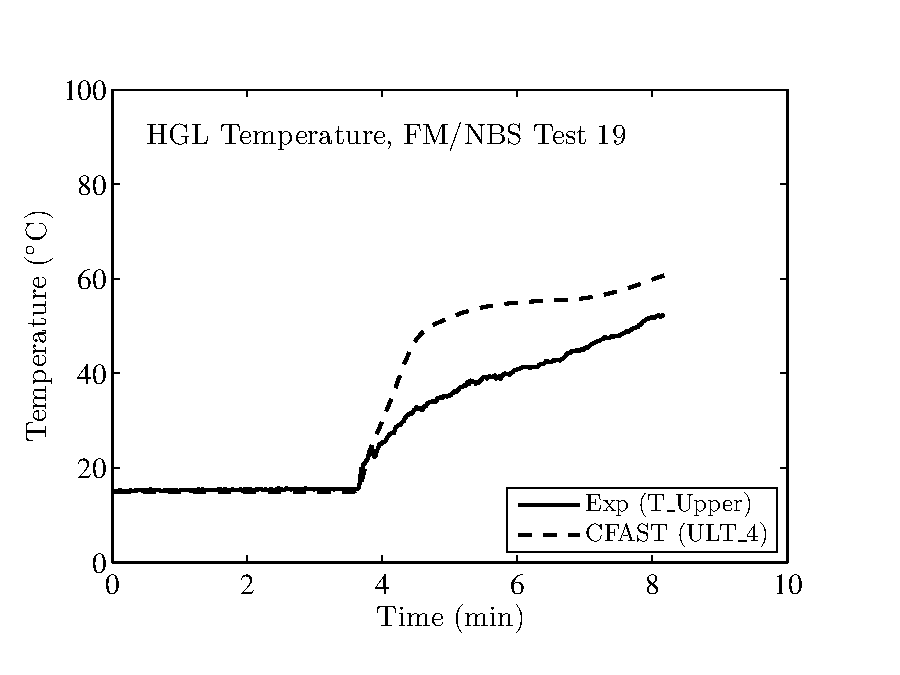
\includegraphics[width=2.6in]{FIGURES/FM_NBS/FM19_4_HGL_Temp} &
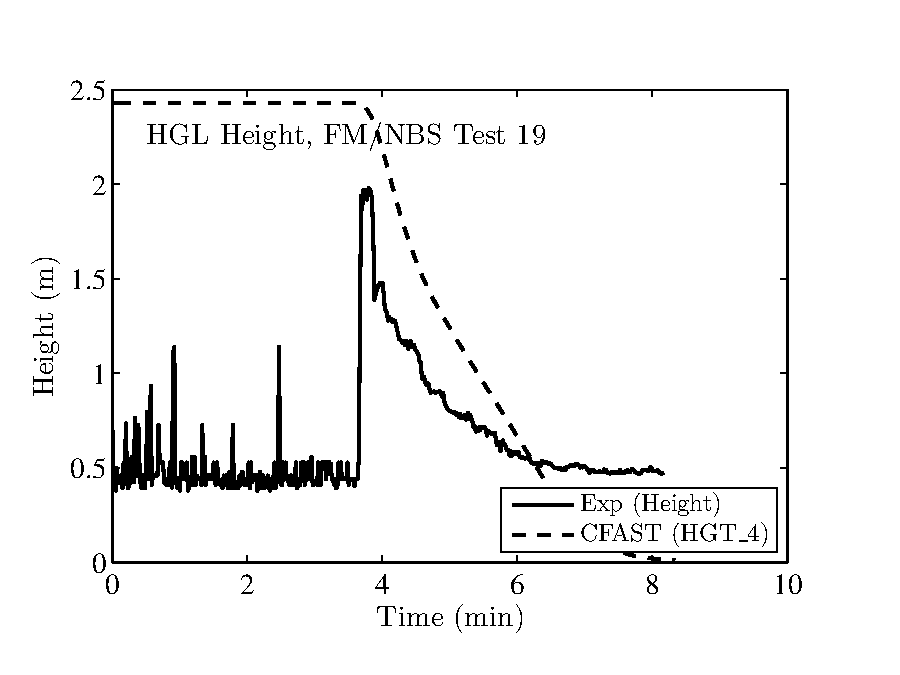
\includegraphics[width=2.6in]{FIGURES/FM_NBS/FM19_4_HGL_Height} \\
\end{tabular*}
\end{figure}

\begin{figure}[p]
\begin{tabular*}{\textwidth}{l@{\extracolsep{\fill}}r}
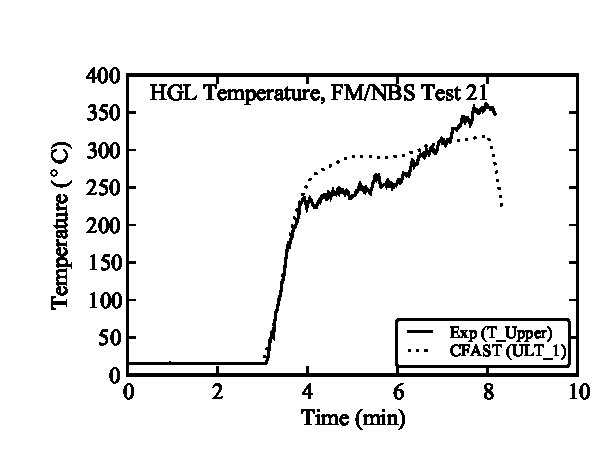
\includegraphics[width=2.6in]{FIGURES/FM_NBS/FM21_1_HGL_Temp} &
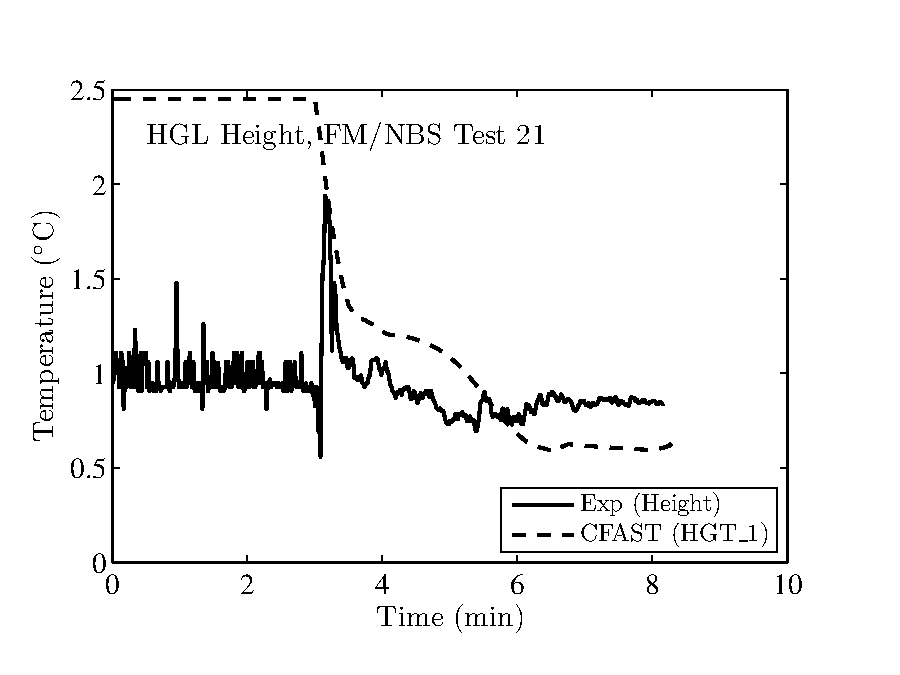
\includegraphics[width=2.6in]{FIGURES/FM_NBS/FM21_1_HGL_Height} \\
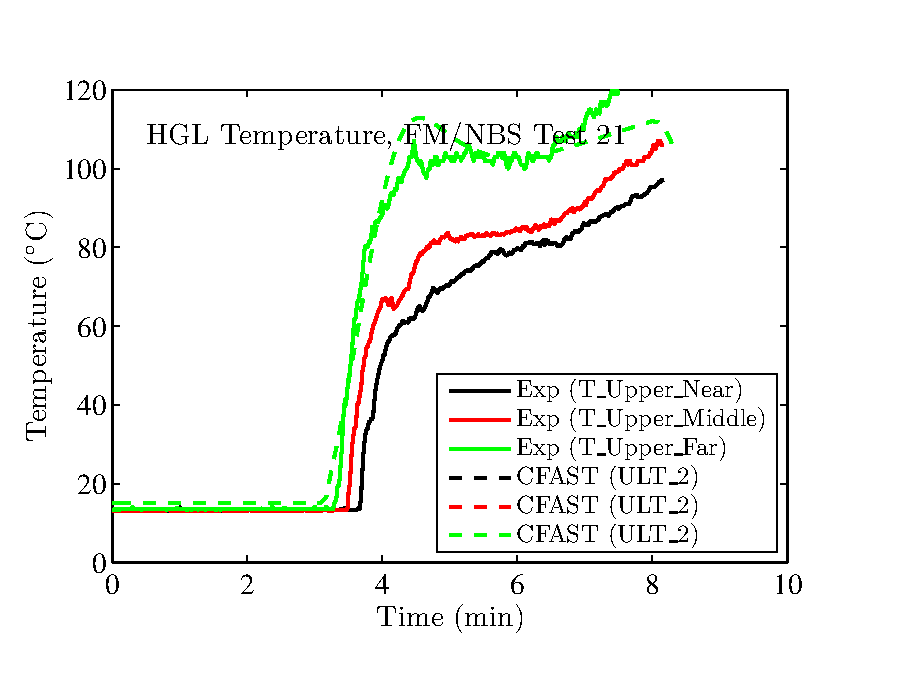
\includegraphics[width=2.6in]{FIGURES/FM_NBS/FM21_2_HGL_Temp} &
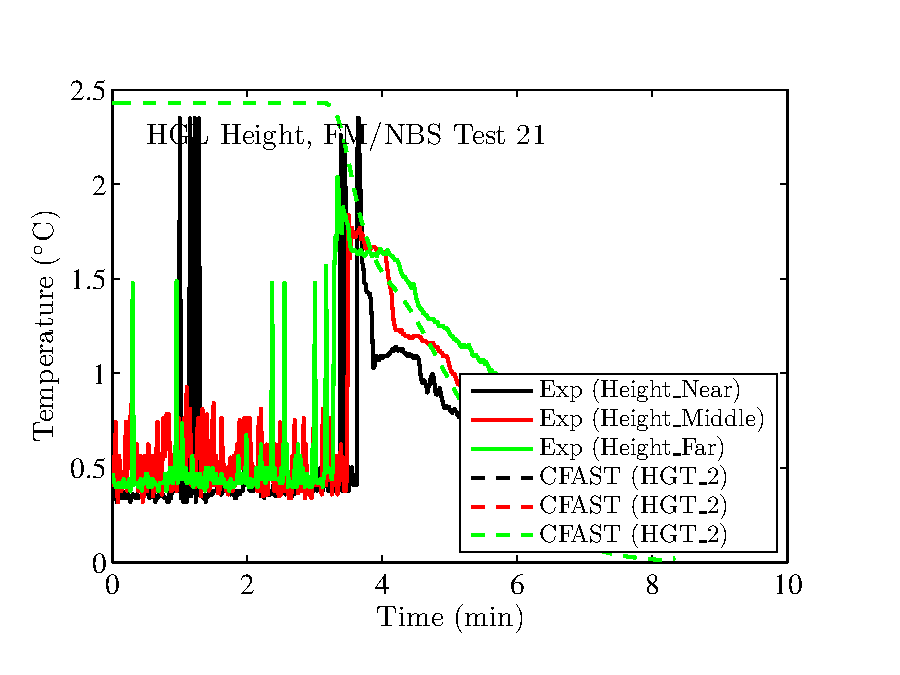
\includegraphics[width=2.6in]{FIGURES/FM_NBS/FM21_2_HGL_Height} \\
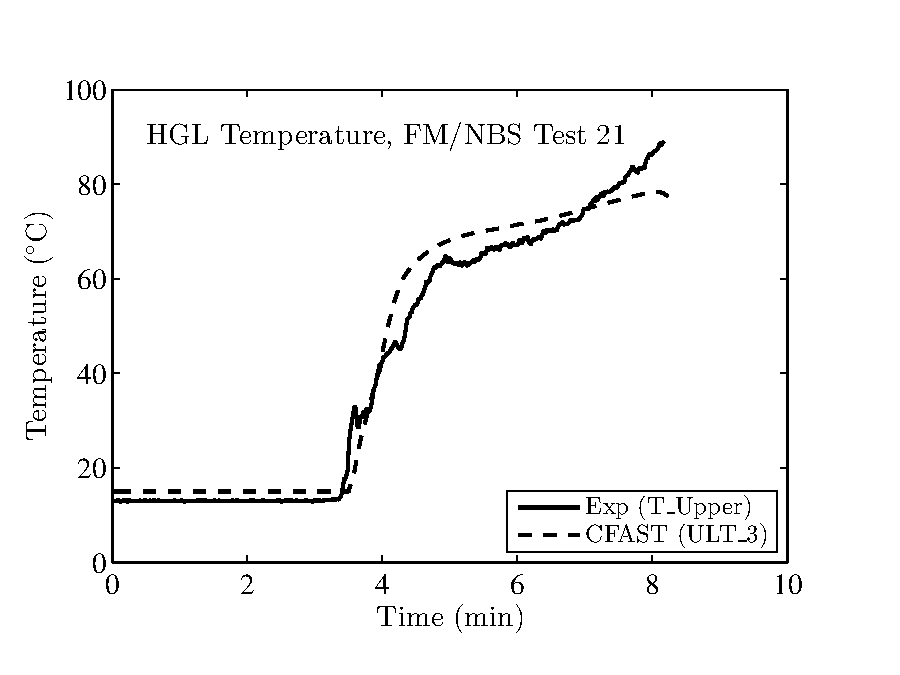
\includegraphics[width=2.6in]{FIGURES/FM_NBS/FM21_3_HGL_Temp} &
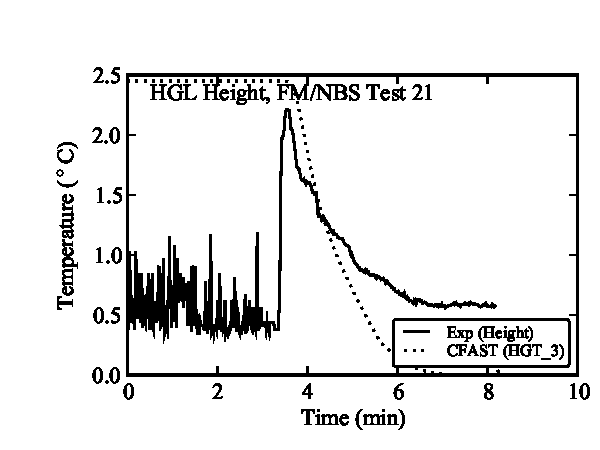
\includegraphics[width=2.6in]{FIGURES/FM_NBS/FM21_3_HGL_Height} \\
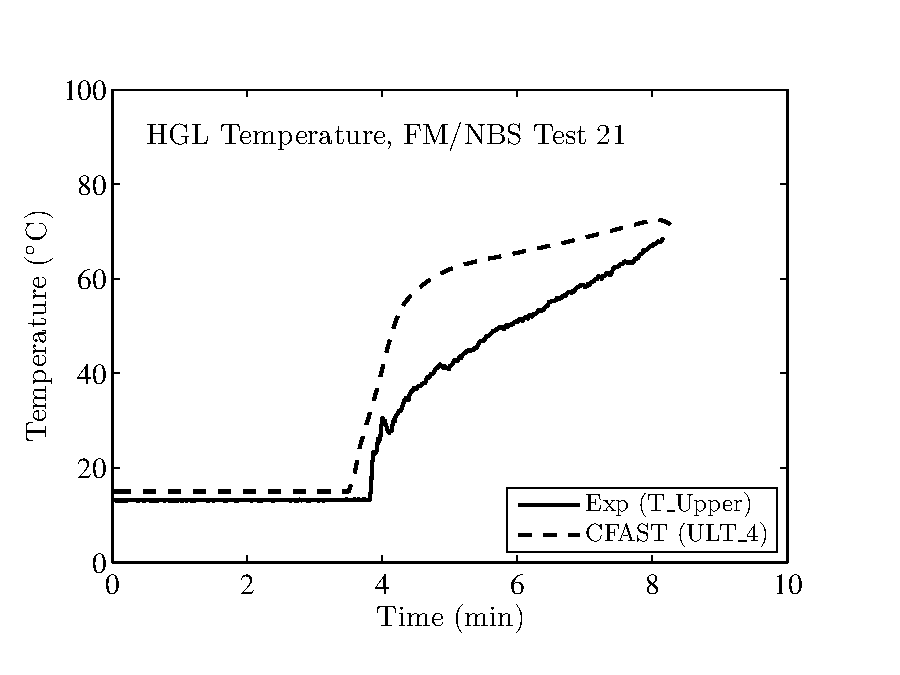
\includegraphics[width=2.6in]{FIGURES/FM_NBS/FM21_4_HGL_Temp} &
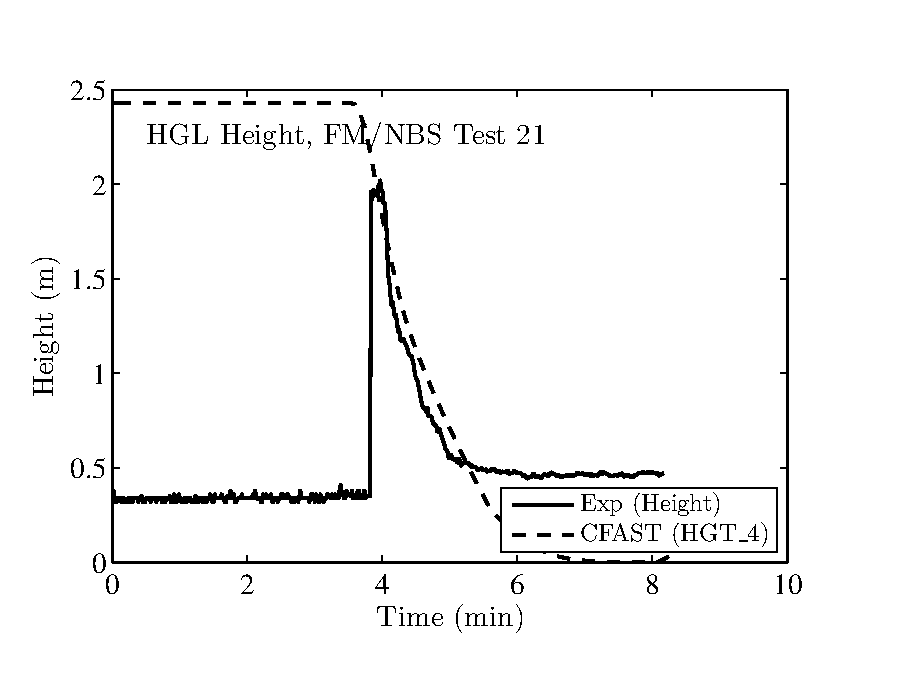
\includegraphics[width=2.6in]{FIGURES/FM_NBS/FM21_4_HGL_Height}
\end{tabular*}
\end{figure}

\begin{figure}[p]
\begin{tabular*}{\textwidth}{l@{\extracolsep{\fill}}r}
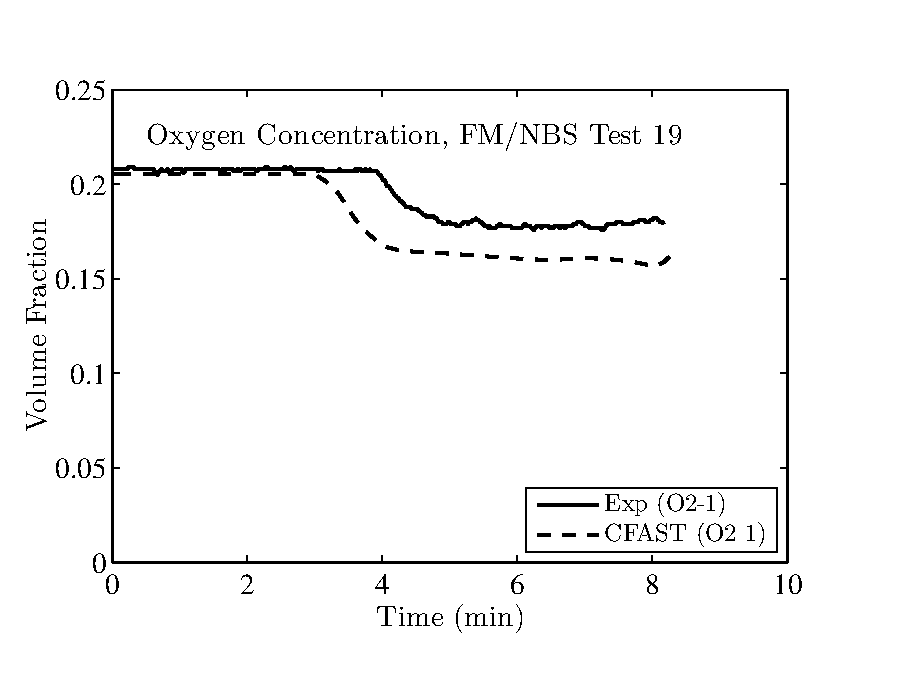
\includegraphics[width=2.6in]{FIGURES/FM_NBS/FM19_1_Oxygen} &
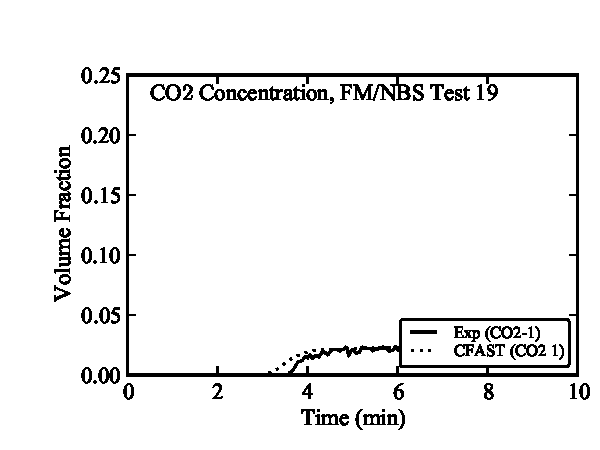
\includegraphics[width=2.6in]{FIGURES/FM_NBS/FM19_1_CO2} \\
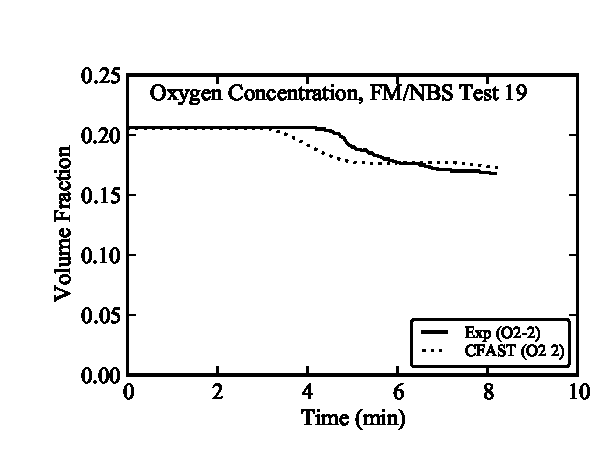
\includegraphics[width=2.6in]{FIGURES/FM_NBS/FM19_2_Oxygen} &
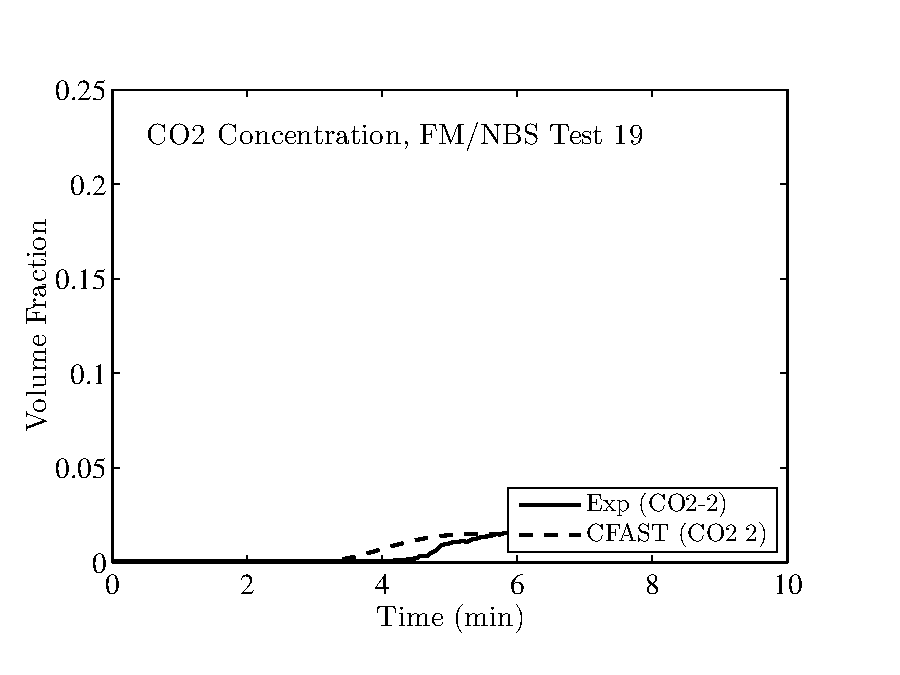
\includegraphics[width=2.6in]{FIGURES/FM_NBS/FM19_2_CO2} \\
 &
\includegraphics[width=2.6in]{FIGURES/FM_NBS/FM19_3_CO2} \\
&
\includegraphics[width=2.6in]{FIGURES/FM_NBS/FM19_4_CO2}
\end{tabular*}
\end{figure}

\begin{figure}[p]
\begin{tabular*}{\textwidth}{l@{\extracolsep{\fill}}r}
\includegraphics[width=2.6in]{FIGURES/FM_NBS/FM21_1_Oxygen} &
\includegraphics[width=2.6in]{FIGURES/FM_NBS/FM21_1_CO2} \\
\includegraphics[width=2.6in]{FIGURES/FM_NBS/FM21_2_Oxygen} &
\includegraphics[width=2.6in]{FIGURES/FM_NBS/FM21_2_CO2} \\
 &
\includegraphics[width=2.6in]{FIGURES/FM_NBS/FM21_3_CO2} \\
&
\includegraphics[width=2.6in]{FIGURES/FM_NBS/FM21_4_CO2}
\end{tabular*}
\end{figure}

\clearpage

\section{FM/SNL Test Series}

The Factory Mutual and Sandia National Laboratories (FM/SNL) Test Series was a series of 25 fire tests conducted in 1985 for the NRC by Factory Mutual Research Corporation (FMRC), under the direction of Sandia National Laboratories (SNL).  The primary purpose of these tests was to provide data with which to validate computer models for various types of NPP compartments.  The experiments were conducted in an enclosure measuring 18 m x 12 m x 6 m, constructed at the FMRC fire test facility in Rhode Island.  The FM/SNL test series is described in detail, including the types and locations of measurement devices, as well as some results in References \cite{Nowlen:1987, Sandia:1989}.

\begin{figure}[p]
\begin{tabular*}{\textwidth}{l@{\extracolsep{\fill}}r}
\includegraphics[width=2.6in]{FIGURES/FM_SNL/FM_SNL_01_HGL_Temp} &
\includegraphics[width=2.6in]{FIGURES/FM_SNL/FM_SNL_01_HGL_Height} \\
\includegraphics[width=2.6in]{FIGURES/FM_SNL/FM_SNL_02_HGL_Temp} &
\includegraphics[width=2.6in]{FIGURES/FM_SNL/FM_SNL_02_HGL_Height} \\
\includegraphics[width=2.6in]{FIGURES/FM_SNL/FM_SNL_03_HGL_Temp} &
\includegraphics[width=2.6in]{FIGURES/FM_SNL/FM_SNL_03_HGL_Height} \\
\includegraphics[width=2.6in]{FIGURES/FM_SNL/FM_SNL_04_HGL_Temp} &
\includegraphics[width=2.6in]{FIGURES/FM_SNL/FM_SNL_04_HGL_Height}
\end{tabular*}
\end{figure}

\begin{figure}[p]
\begin{tabular*}{\textwidth}{l@{\extracolsep{\fill}}r}
\includegraphics[width=2.6in]{FIGURES/FM_SNL/FM_SNL_05_HGL_Temp} &
\includegraphics[width=2.6in]{FIGURES/FM_SNL/FM_SNL_05_HGL_Height} \\\includegraphics[width=2.6in]{FIGURES/FM_SNL/FM_SNL_06_HGL_Temp} &
\includegraphics[width=2.6in]{FIGURES/FM_SNL/FM_SNL_06_HGL_Height} \\
\includegraphics[width=2.6in]{FIGURES/FM_SNL/FM_SNL_07_HGL_Temp} &
\includegraphics[width=2.6in]{FIGURES/FM_SNL/FM_SNL_07_HGL_Height} \\
\includegraphics[width=2.6in]{FIGURES/FM_SNL/FM_SNL_08_HGL_Temp} &
\includegraphics[width=2.6in]{FIGURES/FM_SNL/FM_SNL_08_HGL_Height}
\end{tabular*}
\end{figure}

\begin{figure}[p]
\begin{tabular*}{\textwidth}{l@{\extracolsep{\fill}}r}
\includegraphics[width=2.6in]{FIGURES/FM_SNL/FM_SNL_09_HGL_Temp} &
\includegraphics[width=2.6in]{FIGURES/FM_SNL/FM_SNL_09_HGL_Height} \\\includegraphics[width=2.6in]{FIGURES/FM_SNL/FM_SNL_10_HGL_Temp} &
\includegraphics[width=2.6in]{FIGURES/FM_SNL/FM_SNL_10_HGL_Height} \\
\includegraphics[width=2.6in]{FIGURES/FM_SNL/FM_SNL_11_HGL_Temp} &
\includegraphics[width=2.6in]{FIGURES/FM_SNL/FM_SNL_11_HGL_Height} \\
\includegraphics[width=2.6in]{FIGURES/FM_SNL/FM_SNL_12_HGL_Temp} &
\includegraphics[width=2.6in]{FIGURES/FM_SNL/FM_SNL_12_HGL_Height}
\end{tabular*}
\end{figure}

\begin{figure}[p]
\begin{tabular*}{\textwidth}{l@{\extracolsep{\fill}}r}
\includegraphics[width=2.6in]{FIGURES/FM_SNL/FM_SNL_13_HGL_Temp} &
\includegraphics[width=2.6in]{FIGURES/FM_SNL/FM_SNL_13_HGL_Height} \\
\includegraphics[width=2.6in]{FIGURES/FM_SNL/FM_SNL_14_HGL_Temp} &
\includegraphics[width=2.6in]{FIGURES/FM_SNL/FM_SNL_14_HGL_Height} \\
\includegraphics[width=2.6in]{FIGURES/FM_SNL/FM_SNL_15_HGL_Temp} &
\includegraphics[width=2.6in]{FIGURES/FM_SNL/FM_SNL_15_HGL_Height} \\
\includegraphics[width=2.6in]{FIGURES/FM_SNL/FM_SNL_16_HGL_Temp} &
\includegraphics[width=2.6in]{FIGURES/FM_SNL/FM_SNL_16_HGL_Height}
\end{tabular*}\end{figure}

\begin{figure}[p]
\begin{tabular*}{\textwidth}{l@{\extracolsep{\fill}}r}
\includegraphics[width=2.6in]{FIGURES/FM_SNL/FM_SNL_17_HGL_Temp} &
\includegraphics[width=2.6in]{FIGURES/FM_SNL/FM_SNL_17_HGL_Height} \\
\includegraphics[width=2.6in]{FIGURES/FM_SNL/FM_SNL_21_HGL_Temp} &
\includegraphics[width=2.6in]{FIGURES/FM_SNL/FM_SNL_21_HGL_Height} \\
\includegraphics[width=2.6in]{FIGURES/FM_SNL/FM_SNL_22_HGL_Temp} &
\includegraphics[width=2.6in]{FIGURES/FM_SNL/FM_SNL_22_HGL_Height}
\end{tabular*}
\end{figure}

\begin{figure}[p]
\begin{tabular*}{\textwidth}{l@{\extracolsep{\fill}}r}
\includegraphics[width=2.6in]{FIGURES/FM_SNL/FM_SNL_01_Plume_Temperature} &
\includegraphics[width=2.6in]{FIGURES/FM_SNL/FM_SNL_02_Plume_Temperature} \\
\includegraphics[width=2.6in]{FIGURES/FM_SNL/FM_SNL_03_Plume_Temperature} &
\includegraphics[width=2.6in]{FIGURES/FM_SNL/FM_SNL_04_Plume_Temperature} \\
\includegraphics[width=2.6in]{FIGURES/FM_SNL/FM_SNL_05_Plume_Temperature} &
\includegraphics[width=2.6in]{FIGURES/FM_SNL/FM_SNL_06_Plume_Temperature} \\
\includegraphics[width=2.6in]{FIGURES/FM_SNL/FM_SNL_07_Plume_Temperature} &
\includegraphics[width=2.6in]{FIGURES/FM_SNL/FM_SNL_08_Plume_Temperature}
\end{tabular*}
\end{figure}

\begin{figure}[p]
\begin{tabular*}{\textwidth}{l@{\extracolsep{\fill}}r}
\includegraphics[width=2.6in]{FIGURES/FM_SNL/FM_SNL_09_Plume_Temperature} &
\includegraphics[width=2.6in]{FIGURES/FM_SNL/FM_SNL_10_Plume_Temperature} \\
\includegraphics[width=2.6in]{FIGURES/FM_SNL/FM_SNL_11_Plume_Temperature} &
\includegraphics[width=2.6in]{FIGURES/FM_SNL/FM_SNL_12_Plume_Temperature} \\
\includegraphics[width=2.6in]{FIGURES/FM_SNL/FM_SNL_13_Plume_Temperature} &
\includegraphics[width=2.6in]{FIGURES/FM_SNL/FM_SNL_14_Plume_Temperature} \\
\includegraphics[width=2.6in]{FIGURES/FM_SNL/FM_SNL_15_Plume_Temperature} &
\includegraphics[width=2.6in]{FIGURES/FM_SNL/FM_SNL_16_Plume_Temperature}
\end{tabular*}
\end{figure}

\begin{figure}[p]
\begin{center}
\includegraphics[width=2.6in]{FIGURES/FM_SNL/FM_SNL_17_Plume_Temperature} \\
\includegraphics[width=2.6in]{FIGURES/FM_SNL/FM_SNL_21_Plume_Temperature} \\
\includegraphics[width=2.6in]{FIGURES/FM_SNL/FM_SNL_22_Plume_Temperature}
\end{center}
\end{figure}

\begin{figure}[p]
\begin{tabular*}{\textwidth}{l@{\extracolsep{\fill}}r}
\includegraphics[width=2.6in]{FIGURES/FM_SNL/FM_SNL_01_Ceiling_Jet} &
\includegraphics[width=2.6in]{FIGURES/FM_SNL/FM_SNL_02_Ceiling_Jet} \\
\includegraphics[width=2.6in]{FIGURES/FM_SNL/FM_SNL_03_Ceiling_Jet} &
\includegraphics[width=2.6in]{FIGURES/FM_SNL/FM_SNL_04_Ceiling_Jet} \\
\includegraphics[width=2.6in]{FIGURES/FM_SNL/FM_SNL_05_Ceiling_Jet} &
\includegraphics[width=2.6in]{FIGURES/FM_SNL/FM_SNL_06_Ceiling_Jet} \\
\includegraphics[width=2.6in]{FIGURES/FM_SNL/FM_SNL_07_Ceiling_Jet} &
\includegraphics[width=2.6in]{FIGURES/FM_SNL/FM_SNL_08_Ceiling_Jet}
\end{tabular*}
\end{figure}

\begin{figure}[p]
\begin{tabular*}{\textwidth}{l@{\extracolsep{\fill}}r}
\includegraphics[width=2.6in]{FIGURES/FM_SNL/FM_SNL_09_Ceiling_Jet} &
\includegraphics[width=2.6in]{FIGURES/FM_SNL/FM_SNL_10_Ceiling_Jet} \\
\includegraphics[width=2.6in]{FIGURES/FM_SNL/FM_SNL_11_Ceiling_Jet} &
\includegraphics[width=2.6in]{FIGURES/FM_SNL/FM_SNL_12_Ceiling_Jet} \\
\includegraphics[width=2.6in]{FIGURES/FM_SNL/FM_SNL_13_Ceiling_Jet} &
\includegraphics[width=2.6in]{FIGURES/FM_SNL/FM_SNL_14_Ceiling_Jet} \\
\includegraphics[width=2.6in]{FIGURES/FM_SNL/FM_SNL_15_Ceiling_Jet} &
\includegraphics[width=2.6in]{FIGURES/FM_SNL/FM_SNL_16_Ceiling_Jet}
\end{tabular*}
\end{figure}

\begin{figure}[p]
\begin{center}
\includegraphics[width=2.6in]{FIGURES/FM_SNL/FM_SNL_17_Ceiling_Jet} \\
\includegraphics[width=2.6in]{FIGURES/FM_SNL/FM_SNL_21_Ceiling_Jet} \\
\includegraphics[width=2.6in]{FIGURES/FM_SNL/FM_SNL_22_Ceiling_Jet}
\end{center}
\end{figure}

\clearpage

\section{iBMB Compartment Tests}

A series of small compartment kerosene pool fire experiments, conducted at the
Institut f\"ur Baustoffe, Massivbau und Brandschutz (iBMB) of Braunschweig University of
Technology in Germany in 2004 \cite{Klein-Helbetaling:2005}.  The results from Test 1 were
considered here.  These experiments involved relatively large fires in a relatively small (3.6 m x 3.6 m x 5.7 m) concrete enclosure.

A second series of fire experiments in 2004, conducted under the International Collaborative Fire Model Project (ICFMP) involved realistically routed cable
trays inside the same concrete enclosure at iBMB \cite{Riese:2004}. The compartment was configured slightly differently with a ceiling height of 5.6 m.

Temperature measurements conducted during the test series were used to estimate the HGL temperature and depth.


\begin{figure}[p]
\begin{tabular*}{\textwidth}{l@{\extracolsep{\fill}}r}
\includegraphics[width=2.6in]{FIGURES/iBMB/iBMB_Pool_HGL_Temp} &
\includegraphics[width=2.6in]{FIGURES/iBMB/iBMB_Pool_HGL_Height} \\
\includegraphics[width=2.6in]{FIGURES/iBMB/iBMB_Cable_HGL_Temp} &
\includegraphics[width=2.6in]{FIGURES/iBMB/iBMB_Cable_HGL_Height}
\end{tabular*}
\end{figure}

\clearpage

\section{LLNL Enclosure Series}

The plots on the following pages compare predicted and measured layer temperatures from the LLNL Enclosure test series. In the experiments, fifteen thermocouples were evenly spaced from floor to ceiling on either side of the burner. The measured temperatures were reported as averages of the lower, middle, and upper five TCs. Some of the experiments were conducted with a separated plenum space in the top one-third of the overall compartment (Tests~17-60). In these cases, the upper five TCs are a measure of the average plenum temperature.

In the figures on the following pages, the black circles represent the average of the five upper-most TC measurements. The lines represent the simulation. The red circles represent the average of the middle five TC measurements. For the plenum tests, these TCs are located immediately beneath the plenum and their average temperature is typically greater than that of the plenum. Note that in a number of tests, the fuel flow was stopped or the fire self-extinguished. The simulations last only as long as the reported measurements.

\begin{figure}[p]
\begin{tabular*}{\textwidth}{l@{\extracolsep{\fill}}r}
\includegraphics[width=2.6in]{FIGURES/LLNL_Enclosure/LLNL_01_Temp} &
\includegraphics[width=2.6in]{FIGURES/LLNL_Enclosure/LLNL_02_Temp} \\
\includegraphics[width=2.6in]{FIGURES/LLNL_Enclosure/LLNL_03_Temp} &
\includegraphics[width=2.6in]{FIGURES/LLNL_Enclosure/LLNL_04_Temp} \\
\includegraphics[width=2.6in]{FIGURES/LLNL_Enclosure/LLNL_05_Temp} &
\includegraphics[width=2.6in]{FIGURES/LLNL_Enclosure/LLNL_06_Temp} \\
\includegraphics[width=2.6in]{FIGURES/LLNL_Enclosure/LLNL_07_Temp} &
\includegraphics[width=2.6in]{FIGURES/LLNL_Enclosure/LLNL_08_Temp}
\end{tabular*}
\label{LLNL_Enclosure_Temp_1}
\end{figure}

\begin{figure}[p]
\begin{tabular*}{\textwidth}{l@{\extracolsep{\fill}}r}
\includegraphics[width=2.6in]{FIGURES/LLNL_Enclosure/LLNL_09_Temp} &
\includegraphics[width=2.6in]{FIGURES/LLNL_Enclosure/LLNL_10_Temp} \\
\includegraphics[width=2.6in]{FIGURES/LLNL_Enclosure/LLNL_11_Temp} &
\includegraphics[width=2.6in]{FIGURES/LLNL_Enclosure/LLNL_12_Temp} \\
\includegraphics[width=2.6in]{FIGURES/LLNL_Enclosure/LLNL_13_Temp} &
\includegraphics[width=2.6in]{FIGURES/LLNL_Enclosure/LLNL_14_Temp} \\
 \includegraphics[width=2.6in]{FIGURES/LLNL_Enclosure/LLNL_15_Temp} &
\includegraphics[width=2.6in]{FIGURES/LLNL_Enclosure/LLNL_16_Temp}
\end{tabular*}
\label{LLNL_Enclosure_Temp_2}
\end{figure}

\begin{figure}[p]
\begin{tabular*}{\textwidth}{l@{\extracolsep{\fill}}r}
 \includegraphics[width=2.6in]{FIGURES/LLNL_Enclosure/LLNL_17_Temp} &
 \includegraphics[width=2.6in]{FIGURES/LLNL_Enclosure/LLNL_18_Temp} \\
\includegraphics[width=2.6in]{FIGURES/LLNL_Enclosure/LLNL_19_Temp} &
 \includegraphics[width=2.6in]{FIGURES/LLNL_Enclosure/LLNL_20_Temp} \\
\includegraphics[width=2.6in]{FIGURES/LLNL_Enclosure/LLNL_21_Temp} &
\includegraphics[width=2.6in]{FIGURES/LLNL_Enclosure/LLNL_22_Temp} \\
\includegraphics[width=2.6in]{FIGURES/LLNL_Enclosure/LLNL_23_Temp} &
\includegraphics[width=2.6in]{FIGURES/LLNL_Enclosure/LLNL_24_Temp}
\end{tabular*}
\label{LLNL_Enclosure_Temp_3}
\end{figure}

\begin{figure}[p]
\begin{tabular*}{\textwidth}{l@{\extracolsep{\fill}}r}
\includegraphics[width=2.6in]{FIGURES/LLNL_Enclosure/LLNL_25_Temp} &
\includegraphics[width=2.6in]{FIGURES/LLNL_Enclosure/LLNL_26_Temp} \\
\includegraphics[width=2.6in]{FIGURES/LLNL_Enclosure/LLNL_27_Temp} &
\includegraphics[width=2.6in]{FIGURES/LLNL_Enclosure/LLNL_28_Temp} \\
\includegraphics[width=2.6in]{FIGURES/LLNL_Enclosure/LLNL_29_Temp} &
\includegraphics[width=2.6in]{FIGURES/LLNL_Enclosure/LLNL_30_Temp} \\
\includegraphics[width=2.6in]{FIGURES/LLNL_Enclosure/LLNL_31_Temp} &
\includegraphics[width=2.6in]{FIGURES/LLNL_Enclosure/LLNL_32_Temp}
\end{tabular*}
\label{LLNL_Enclosure_Temp_4}
\end{figure}

\begin{figure}[p]
\begin{tabular*}{\textwidth}{l@{\extracolsep{\fill}}r}
\includegraphics[width=2.6in]{FIGURES/LLNL_Enclosure/LLNL_33_Temp} &
\includegraphics[width=2.6in]{FIGURES/LLNL_Enclosure/LLNL_34_Temp} \\
\includegraphics[width=2.6in]{FIGURES/LLNL_Enclosure/LLNL_35_Temp} &
\includegraphics[width=2.6in]{FIGURES/LLNL_Enclosure/LLNL_36_Temp} \\
\includegraphics[width=2.6in]{FIGURES/LLNL_Enclosure/LLNL_37_Temp} &
\includegraphics[width=2.6in]{FIGURES/LLNL_Enclosure/LLNL_38_Temp} \\
\includegraphics[width=2.6in]{FIGURES/LLNL_Enclosure/LLNL_39_Temp} &
\includegraphics[width=2.6in]{FIGURES/LLNL_Enclosure/LLNL_40_Temp}
\end{tabular*}
\label{LLNL_Enclosure_Temp_5}
\end{figure}

\begin{figure}[p]
\begin{tabular*}{\textwidth}{l@{\extracolsep{\fill}}r}
\includegraphics[width=2.6in]{FIGURES/LLNL_Enclosure/LLNL_41_Temp} &
\includegraphics[width=2.6in]{FIGURES/LLNL_Enclosure/LLNL_42_Temp} \\
\includegraphics[width=2.6in]{FIGURES/LLNL_Enclosure/LLNL_43_Temp} &
\includegraphics[width=2.6in]{FIGURES/LLNL_Enclosure/LLNL_44_Temp} \\
\includegraphics[width=2.6in]{FIGURES/LLNL_Enclosure/LLNL_45_Temp} &
\includegraphics[width=2.6in]{FIGURES/LLNL_Enclosure/LLNL_46_Temp} \\
\includegraphics[width=2.6in]{FIGURES/LLNL_Enclosure/LLNL_47_Temp} &
\includegraphics[width=2.6in]{FIGURES/LLNL_Enclosure/LLNL_48_Temp}
\end{tabular*}
\label{LLNL_Enclosure_Temp_6}
\end{figure}

\begin{figure}[p]
\begin{tabular*}{\textwidth}{l@{\extracolsep{\fill}}r}
\includegraphics[width=2.6in]{FIGURES/LLNL_Enclosure/LLNL_49_Temp} &
\includegraphics[width=2.6in]{FIGURES/LLNL_Enclosure/LLNL_50_Temp} \\
\includegraphics[width=2.6in]{FIGURES/LLNL_Enclosure/LLNL_51_Temp} &
\includegraphics[width=2.6in]{FIGURES/LLNL_Enclosure/LLNL_52_Temp} \\
\includegraphics[width=2.6in]{FIGURES/LLNL_Enclosure/LLNL_53_Temp} &
\includegraphics[width=2.6in]{FIGURES/LLNL_Enclosure/LLNL_54_Temp} \\
\includegraphics[width=2.6in]{FIGURES/LLNL_Enclosure/LLNL_55_Temp} &
\includegraphics[width=2.6in]{FIGURES/LLNL_Enclosure/LLNL_56_Temp}
\end{tabular*}
\label{LLNL_Enclosure_Temp_7}
\end{figure}

\begin{figure}[p]
\begin{tabular*}{\textwidth}{l@{\extracolsep{\fill}}r}
\includegraphics[width=2.6in]{FIGURES/LLNL_Enclosure/LLNL_57_Temp} &
\includegraphics[width=2.6in]{FIGURES/LLNL_Enclosure/LLNL_58_Temp} \\
\includegraphics[width=2.6in]{FIGURES/LLNL_Enclosure/LLNL_59_Temp} &
\includegraphics[width=2.6in]{FIGURES/LLNL_Enclosure/LLNL_60_Temp} \\
\includegraphics[width=2.6in]{FIGURES/LLNL_Enclosure/LLNL_61_Temp} &
\includegraphics[width=2.6in]{FIGURES/LLNL_Enclosure/LLNL_62_Temp} \\
\includegraphics[width=2.6in]{FIGURES/LLNL_Enclosure/LLNL_63_Temp} &
\includegraphics[width=2.6in]{FIGURES/LLNL_Enclosure/LLNL_64_Temp}
\end{tabular*}
\label{LLNL_Enclosure_Temp_8}
\end{figure}

\clearpage

The test report of the LLNL Enclosure experiments lists the mass flow rate, $\dot{m}$, through the exhaust duct at different times during the tests. It also lists the compartment pressures, $\Delta p$, at these same times. From the simple leak formula:
\be
   \frac{\dot{m}}{\rho_0} = A \, \sqrt{\frac{2 \, \Delta p}{\rho_0}}
\ee
the leakage area, $A$, is estimated to be 0.018~m$^2$, based on the initial exhaust rate and pressure. For modeling purposes, the ``leakage area'' is assumed to be the sum of the inlet duct area plus any actual compartment leakage area. The mass flow rate through the exhaust duct is specified explicitly in the model. The test report does not provide enough information about the ventilation system to model the fan and filtration system within the exhaust duct.

In the figures on the following pages, the open circles represent the measured pressure; the line represents the predicted pressure. The predicted pressures are time-averaged over a time interval that is one-tenth the total simulation time. In general, the short-duration pressure spike that is typical of fires within relatively tight compartments has been smoothed over in the reported test data. Depending on the simulation, it often appears in the simulation data. The comparison of measurement and prediction is based on the final few pressure points, not the initial spike.

Only some of the 64 experiments are included. In some cases, the fan was turned off and there is not enough information in the test report to determine the pressure losses through the duct. In other cases, there are only two pressure measurements reported; one at the start of the test, the other either before or after extinction. In various other cases, either there is not enough data or the data is inconsistent with the reported conditions. For cases where the door to the compartment was open, the measured gauge pressures at the start of the experiment ranged from 0~Pa to 10~Pa. There is not enough information in the test report to explain why the starting pressures were not 0~Pa; thus, the measured pressures were adjusted so that the starting pressure is 0~Pa.

\begin{figure}[p]
\begin{tabular*}{\textwidth}{l@{\extracolsep{\fill}}r}
\includegraphics[height=2.2in]{FIGURES/LLNL_Enclosure/LLNL_09_Pres} &
\includegraphics[height=2.2in]{FIGURES/LLNL_Enclosure/LLNL_11_Pres} \\
\includegraphics[height=2.2in]{FIGURES/LLNL_Enclosure/LLNL_12_Pres} &
\includegraphics[height=2.2in]{FIGURES/LLNL_Enclosure/LLNL_13_Pres} \\
\includegraphics[height=2.2in]{FIGURES/LLNL_Enclosure/LLNL_14_Pres} &
\includegraphics[height=2.2in]{FIGURES/LLNL_Enclosure/LLNL_15_Pres} \\
\includegraphics[height=2.2in]{FIGURES/LLNL_Enclosure/LLNL_16_Pres} &
\includegraphics[height=2.2in]{FIGURES/LLNL_Enclosure/LLNL_17_Pres}
\end{tabular*}
\label{LLNL_Enclosure_Pres_2}
\end{figure}

\begin{figure}[p]
\begin{tabular*}{\textwidth}{l@{\extracolsep{\fill}}r}
\includegraphics[height=2.2in]{FIGURES/LLNL_Enclosure/LLNL_18_Pres} &
\includegraphics[height=2.2in]{FIGURES/LLNL_Enclosure/LLNL_19_Pres} \\
\includegraphics[height=2.2in]{FIGURES/LLNL_Enclosure/LLNL_20_Pres} &
\includegraphics[height=2.2in]{FIGURES/LLNL_Enclosure/LLNL_23_Pres} \\
\includegraphics[height=2.2in]{FIGURES/LLNL_Enclosure/LLNL_26_Pres} &
\includegraphics[height=2.2in]{FIGURES/LLNL_Enclosure/LLNL_29_Pres} \\
\includegraphics[height=2.2in]{FIGURES/LLNL_Enclosure/LLNL_30_Pres} &
\includegraphics[height=2.2in]{FIGURES/LLNL_Enclosure/LLNL_31_Pres}
\end{tabular*}
\label{LLNL_Enclosure_Pres_3}
\end{figure}

\begin{figure}[p]
\begin{tabular*}{\textwidth}{l@{\extracolsep{\fill}}r}
\includegraphics[height=2.2in]{FIGURES/LLNL_Enclosure/LLNL_32_Pres} &
\includegraphics[height=2.2in]{FIGURES/LLNL_Enclosure/LLNL_33_Pres} \\
\includegraphics[height=2.2in]{FIGURES/LLNL_Enclosure/LLNL_34_Pres} &
\includegraphics[height=2.2in]{FIGURES/LLNL_Enclosure/LLNL_35_Pres} \\
\includegraphics[height=2.2in]{FIGURES/LLNL_Enclosure/LLNL_36_Pres} &
\includegraphics[height=2.2in]{FIGURES/LLNL_Enclosure/LLNL_38_Pres} \\
\includegraphics[height=2.2in]{FIGURES/LLNL_Enclosure/LLNL_40_Pres} &
\includegraphics[height=2.2in]{FIGURES/LLNL_Enclosure/LLNL_42_Pres}
\end{tabular*}
\label{LLNL_Enclosure_Pres_4}
\end{figure}

\begin{figure}[p]
\begin{tabular*}{\textwidth}{l@{\extracolsep{\fill}}r}
\includegraphics[height=2.2in]{FIGURES/LLNL_Enclosure/LLNL_44_Pres} &
\includegraphics[height=2.2in]{FIGURES/LLNL_Enclosure/LLNL_50_Pres} \\
\includegraphics[height=2.2in]{FIGURES/LLNL_Enclosure/LLNL_51_Pres} &
\includegraphics[height=2.2in]{FIGURES/LLNL_Enclosure/LLNL_52_Pres} \\
\includegraphics[height=2.2in]{FIGURES/LLNL_Enclosure/LLNL_54_Pres} &
\includegraphics[height=2.2in]{FIGURES/LLNL_Enclosure/LLNL_55_Pres} \\
\includegraphics[height=2.2in]{FIGURES/LLNL_Enclosure/LLNL_57_Pres} &
\includegraphics[height=2.2in]{FIGURES/LLNL_Enclosure/LLNL_58_Pres}
\end{tabular*}
\label{LLNL_Enclosure_Pres_5}
\end{figure}

\begin{figure}[p]
\begin{tabular*}{\textwidth}{l@{\extracolsep{\fill}}r}
\includegraphics[height=2.2in]{FIGURES/LLNL_Enclosure/LLNL_59_Pres} &
\includegraphics[height=2.2in]{FIGURES/LLNL_Enclosure/LLNL_60_Pres} \\
\includegraphics[height=2.2in]{FIGURES/LLNL_Enclosure/LLNL_61_Pres} &
\includegraphics[height=2.2in]{FIGURES/LLNL_Enclosure/LLNL_62_Pres} \\
\includegraphics[height=2.2in]{FIGURES/LLNL_Enclosure/LLNL_63_Pres} &
\includegraphics[height=2.2in]{FIGURES/LLNL_Enclosure/LLNL_64_Pres}
\end{tabular*}
\label{LLNL_Enclosure_Pres_6}
\end{figure}


\clearpage

\section{NBS Single Room Tests with Furniture}

These data describe a series of room fire tests using upholstered furniture items in a room of fixed size but with varying opening sizes and shapes \cite{Valid:Babrauskas_Flashover} conducted by the National Bureau of Standards (NBS, former name of NIST). It was selected for its well characterized and realistic fuel sources in a simple single-room geometry. In addition, the wide variation in opening size should provide challenges for current zone fire models. Peak fire size was about 2.9~MW with a total room volume of 21 m$^3$. A series of four single-room fire tests were conducted using upholstered furniture items for comparison with their free burning behavior, previously determined in a furniture calorimeter.  The experiments were conducted in a single room enclosure; ventilation to the room was provided by window openings of  varying sizes. The room was equipped with an instrumented exhaust collection system outside the window opening.

A second similar test series also utilized a single-room fire test with furniture as the fire source \cite{Lee:1985}. It expanded upon the first data set by adding the phenomenon of wall burning. Peak fire size was about 7 MW. The room size was similar to the first test series.

\begin{figure}
\begin{tabular*}{\textwidth}{l@{\extracolsep{\fill}}r}
\includegraphics[width=2.6in]{FIGURES/NBS/1rfurn1_HGL_Temp} &
\includegraphics[width=2.6in]{FIGURES/NBS/1rfurn1_HGL_Height} \\
\includegraphics[width=2.6in]{FIGURES/NBS/1rfurn6_HGL_Temp} &
\includegraphics[width=2.6in]{FIGURES/NBS/1rfurn6_HGL_Height} \\
\includegraphics[width=2.6in]{FIGURES/NBS/1rwall1_HGL_Temp} &
\includegraphics[width=2.6in]{FIGURES/NBS/1rwall1_HGL_Height}\\
\includegraphics[width=2.6in]{FIGURES/NBS/1rwall2_HGL_Temp} &
\includegraphics[width=2.6in]{FIGURES/NBS/1rwall2_HGL_Height}
\end{tabular*}
\end{figure}

\begin{figure}[p]
\begin{center}
\includegraphics[width=2.6in]{FIGURES/NBS/1rfurn1_Oxygen} \\
\includegraphics[width=2.6in]{FIGURES/NBS/1rfurn6_Oxygen}
\end{center}
\end{figure}

\begin{figure}[p]
\begin{center}
\includegraphics[width=2.6in]{FIGURES/NBS/1rwall1_Pressure} \\
\includegraphics[width=2.6in]{FIGURES/NBS/1rwall2_Pressure}
\end{center}
\end{figure}

\clearpage

\section{NBS Multi-Compartment Test Series}

The National Bureau of Standards (NBS, former name of NIST) Multi-Compartment Test Series consisted of 45 fire tests representing 9 different sets of conditions were conducted in a three-room suite.  The experiments were conducted in 1985 and are described in detail in reference \cite{Peacock:1988}.  The suite consisted of two relatively small rooms, connected via a relatively long corridor. Total volume of the structure was approximately 100 m$^2$. The fire source, a gas burner, was located against the rear wall of one of the small compartments . Fire tests of 100 kW, 300 kW and 500 kW were conducted. For the current  study, three 100 kW fire experiments have been used, including Test 100A from Set 1, Test 100O from Set 2, and Test 100Z from Set 4. For the NBS Multi-room series, Tests 100A, 100O and 100Z were selected for study, because they were constructively used in a previous validation study [\cite{EPRI}, and because these tests had  the steadiest values of measured heat release rate during the steady burning period. The selected data are also available in Reference \cite{EPRI}.

\begin{figure}[p]
\begin{tabular*}{\textwidth}{l@{\extracolsep{\fill}}r}
\includegraphics[width=2.6in]{FIGURES/NBS/NBS_100A_Tree_1_HGL_Temp} &
\includegraphics[width=2.6in]{FIGURES/NBS/NBS_100A_Tree_1_HGL_Height} \\
\includegraphics[width=2.6in]{FIGURES/NBS/NBS_100A_Tree_4_HGL_Temp} &
\includegraphics[width=2.6in]{FIGURES/NBS/NBS_100A_Tree_4_HGL_Height} \\
\includegraphics[width=2.6in]{FIGURES/NBS/NBS_100A_Tree_5_HGL_Temp} &
\includegraphics[width=2.6in]{FIGURES/NBS/NBS_100A_Tree_5_HGL_Height}\\
\includegraphics[width=2.6in]{FIGURES/NBS/NBS_100A_Tree_6_HGL_Temp} &
\includegraphics[width=2.6in]{FIGURES/NBS/NBS_100A_Tree_6_HGL_Height}
\end{tabular*}
\end{figure}

\begin{figure}[p]
\begin{tabular*}{\textwidth}{l@{\extracolsep{\fill}}r}
\includegraphics[width=2.6in]{FIGURES/NBS/NBS_100O_Tree_1_HGL_Temp} &
\includegraphics[width=2.6in]{FIGURES/NBS/NBS_100O_Tree_1_HGL_Height} \\
\includegraphics[width=2.6in]{FIGURES/NBS/NBS_100O_Tree_4_HGL_Temp} &
\includegraphics[width=2.6in]{FIGURES/NBS/NBS_100O_Tree_4_HGL_Height} \\
\includegraphics[width=2.6in]{FIGURES/NBS/NBS_100O_Tree_5_HGL_Temp} &
\includegraphics[width=2.6in]{FIGURES/NBS/NBS_100O_Tree_5_HGL_Height}\\
\includegraphics[width=2.6in]{FIGURES/NBS/NBS_100O_Tree_6_HGL_Temp} &
\includegraphics[width=2.6in]{FIGURES/NBS/NBS_100O_Tree_6_HGL_Height}
\end{tabular*}
\end{figure}

\begin{figure}[p]
\begin{tabular*}{\textwidth}{l@{\extracolsep{\fill}}r}
\includegraphics[width=2.6in]{FIGURES/NBS/NBS_100Z_Tree_1_HGL_Temp} &
\includegraphics[width=2.6in]{FIGURES/NBS/NBS_100Z_Tree_1_HGL_Height} \\
\includegraphics[width=2.6in]{FIGURES/NBS/NBS_100Z_Tree_4_HGL_Temp} &
\includegraphics[width=2.6in]{FIGURES/NBS/NBS_100Z_Tree_4_HGL_Height} \\
\includegraphics[width=2.6in]{FIGURES/NBS/NBS_100Z_Tree_5_HGL_Temp} &
\includegraphics[width=2.6in]{FIGURES/NBS/NBS_100Z_Tree_5_HGL_Height}\\
\includegraphics[width=2.6in]{FIGURES/NBS/NBS_100Z_Tree_7_HGL_Temp} &
\includegraphics[width=2.6in]{FIGURES/NBS/NBS_100Z_Tree_7_HGL_Height}
\end{tabular*}
\end{figure}

\clearpage

\section{NIST Smoke Alarm Experiments}

The primary purpose of the NIST smoke alarmexperiments was to measure smoke alarm activation times in residential settings. In the single-story manufactured home tests that were selected for validation, five smoke alarm measurement stations (A-E) were located in different areas of the manufactured home. Included is a scatterplot of measured and predicted smoke alarm activation time. Thermocouple trees were also located at each measurement station. The highest thermocouple in the tree can be compared to ceiling jet temperature predictions. The plots on the following page show the measured and predicted ceiling jet temperatures for the five measurement stations in each test.

\begin{figure}[h!]
\begin{tabular*}{\textwidth}{l@{\extracolsep{\fill}}r}
\includegraphics[width=2.6in]{FIGURES/NIST_Dunes_2000/NIST_Dunes_2000_SDC02_Ceiling_Jet} &
\includegraphics[width=2.6in]{FIGURES/NIST_Dunes_2000/NIST_Dunes_2000_SDC05_Ceiling_Jet} \\
\includegraphics[width=2.6in]{FIGURES/NIST_Dunes_2000/NIST_Dunes_2000_SDC07_Ceiling_Jet} &
\includegraphics[width=2.6in]{FIGURES/NIST_Dunes_2000/NIST_Dunes_2000_SDC10_Ceiling_Jet} \\
\includegraphics[width=2.6in]{FIGURES/NIST_Dunes_2000/NIST_Dunes_2000_SDC33_Ceiling_Jet} &
\includegraphics[width=2.6in]{FIGURES/NIST_Dunes_2000/NIST_Dunes_2000_SDC35_Ceiling_Jet} \\
\includegraphics[width=2.6in]{FIGURES/NIST_Dunes_2000/NIST_Dunes_2000_SDC38_Ceiling_Jet} &
\includegraphics[width=2.6in]{FIGURES/NIST_Dunes_2000/NIST_Dunes_2000_SDC39_Ceiling_Jet}
\end{tabular*}
\label{NIST_Dunes_2000_Ceiling_Jet}
\end{figure}

\clearpage

%\section{NIST Seven-story Hotel Tests}

%By far the most complex test, this data set is part of  a series of full-scale experiments conducted to evaluate zoned smoke control systems, with and without stairwell pressurization \cite{Klote:1990}.  It was conducted in a seven story hotel with multiple rooms on each floor and a stairwell connecting all floors.  This data set was chosen because it would challenge the scope of most current fire models.  Measured temperatures and pressure differences between the rooms and floors of the building are extensive and consistent.  Peak fire size was 3 MW with a total building volume of 140~000 m$^3$. The hotel was a masonry structure consisting of two wings, one three stories and the other seven stories tall. The fires were set on the second floor of the seven-story wing.

%\begin{figure}[p]
%\begin{center}
%\includegraphics[width=2.6in]{FIGURES/NIST_PLAZA/Room_1_HGL_Temp} \\
%\includegraphics[width=2.6in]{FIGURES/NIST_PLAZA/Room_2_HGL_Temp} \\
%\includegraphics[width=2.6in]{FIGURES/NIST_PLAZA/Room_7_HGL_Temp}
%\end{center}
%\end{figure}

%\clearpage

\section{NIST/NRC Test Series}

These experiments, sponsored by the US NRC and conducted at NIST, consisted of 15 large-scale experiments performed in June 2003. All 15 tests were included in the validation study. The experiments are documented in Ref.~\cite{Hamins:2005}. The fire sizes ranged from 350 kW to 2.2 MW in a compartment with dimensions 21.7~m by 7.1~m by 3.8~m high, designed to represent a compartment in a nuclear power plant containing power and control cables. The room had one door and a simple mechanical ventilation system. Ventilation conditions, the fire size, and fire location were varied. Numerous measurements (approximately 350 per test) were made.

\begin{figure}[p]
\begin{tabular*}{\textwidth}{l@{\extracolsep{\fill}}r}
\includegraphics[width=2.6in]{FIGURES/NIST_NRC/NIST_NRC_01_HGL_Temp} &
\includegraphics[width=2.6in]{FIGURES/NIST_NRC/NIST_NRC_01_HGL_Height} \\
\includegraphics[width=2.6in]{FIGURES/NIST_NRC/NIST_NRC_07_HGL_Temp} &
\includegraphics[width=2.6in]{FIGURES/NIST_NRC/NIST_NRC_07_HGL_Height} \\
\includegraphics[width=2.6in]{FIGURES/NIST_NRC/NIST_NRC_02_HGL_Temp} &
\includegraphics[width=2.6in]{FIGURES/NIST_NRC/NIST_NRC_02_HGL_Height} \\
\includegraphics[width=2.6in]{FIGURES/NIST_NRC/NIST_NRC_08_HGL_Temp} &
\includegraphics[width=2.6in]{FIGURES/NIST_NRC/NIST_NRC_08_HGL_Height}
\end{tabular*}
\end{figure}

\begin{figure}[p]
\begin{tabular*}{\textwidth}{l@{\extracolsep{\fill}}r}
\includegraphics[width=2.6in]{FIGURES/NIST_NRC/NIST_NRC_04_HGL_Temp} &
\includegraphics[width=2.6in]{FIGURES/NIST_NRC/NIST_NRC_04_HGL_Height} \\
\includegraphics[width=2.6in]{FIGURES/NIST_NRC/NIST_NRC_10_HGL_Temp} &
\includegraphics[width=2.6in]{FIGURES/NIST_NRC/NIST_NRC_10_HGL_Height} \\
\includegraphics[width=2.6in]{FIGURES/NIST_NRC/NIST_NRC_13_HGL_Temp} &
\includegraphics[width=2.6in]{FIGURES/NIST_NRC/NIST_NRC_13_HGL_Height} \\
\includegraphics[width=2.6in]{FIGURES/NIST_NRC/NIST_NRC_16_HGL_Temp} &
\includegraphics[width=2.6in]{FIGURES/NIST_NRC/NIST_NRC_16_HGL_Height}
\end{tabular*}
\end{figure}

\clearpage

\begin{figure}[p]
\begin{tabular*}{\textwidth}{l@{\extracolsep{\fill}}r}
\includegraphics[width=2.6in]{FIGURES/NIST_NRC/NIST_NRC_17_HGL_Temp} &
\includegraphics[width=2.6in]{FIGURES/NIST_NRC/NIST_NRC_17_HGL_Height} \\
\multicolumn{2}{c}{Open Door Tests to follow} \\
\includegraphics[width=2.6in]{FIGURES/NIST_NRC/NIST_NRC_03_HGL_Temp} &
\includegraphics[width=2.6in]{FIGURES/NIST_NRC/NIST_NRC_03_HGL_Height} \\
\includegraphics[width=2.6in]{FIGURES/NIST_NRC/NIST_NRC_09_HGL_Temp} &
\includegraphics[width=2.6in]{FIGURES/NIST_NRC/NIST_NRC_09_HGL_Height}
\end{tabular*}
\end{figure}

\begin{figure}[p]
\begin{tabular*}{\textwidth}{l@{\extracolsep{\fill}}r}
\includegraphics[width=2.6in]{FIGURES/NIST_NRC/NIST_NRC_05_HGL_Temp} &
\includegraphics[width=2.6in]{FIGURES/NIST_NRC/NIST_NRC_05_HGL_Height} \\
\includegraphics[width=2.6in]{FIGURES/NIST_NRC/NIST_NRC_14_HGL_Temp} &
\includegraphics[width=2.6in]{FIGURES/NIST_NRC/NIST_NRC_14_HGL_Height} \\
\includegraphics[width=2.6in]{FIGURES/NIST_NRC/NIST_NRC_15_HGL_Temp} &
\includegraphics[width=2.6in]{FIGURES/NIST_NRC/NIST_NRC_15_HGL_Height} \\
\includegraphics[width=2.6in]{FIGURES/NIST_NRC/NIST_NRC_18_HGL_Temp} &
\includegraphics[width=2.6in]{FIGURES/NIST_NRC/NIST_NRC_18_HGL_Height}
\end{tabular*}
\end{figure}

\clearpage

\begin{figure}[p]
\begin{tabular*}{\textwidth}{l@{\extracolsep{\fill}}r}
\includegraphics[width=2.6in]{FIGURES/NIST_NRC/NIST_NRC_01_Ceiling_Jet} &
\includegraphics[width=2.6in]{FIGURES/NIST_NRC/NIST_NRC_07_Ceiling_Jet} \\
\includegraphics[width=2.6in]{FIGURES/NIST_NRC/NIST_NRC_02_Ceiling_Jet} &
\includegraphics[width=2.6in]{FIGURES/NIST_NRC/NIST_NRC_08_Ceiling_Jet} \\
\includegraphics[width=2.6in]{FIGURES/NIST_NRC/NIST_NRC_04_Ceiling_Jet} &
\includegraphics[width=2.6in]{FIGURES/NIST_NRC/NIST_NRC_10_Ceiling_Jet} \\
\includegraphics[width=2.6in]{FIGURES/NIST_NRC/NIST_NRC_13_Ceiling_Jet} &
\includegraphics[width=2.6in]{FIGURES/NIST_NRC/NIST_NRC_16_Ceiling_Jet}
\end{tabular*}
\label{NIST_NRC_Jet_Closed}
\end{figure}

\begin{figure}[p]
\begin{tabular*}{\textwidth}{l@{\extracolsep{\fill}}r}
\includegraphics[width=2.6in]{FIGURES/NIST_NRC/NIST_NRC_17_Ceiling_Jet} &
 \\
\includegraphics[width=2.6in]{FIGURES/NIST_NRC/NIST_NRC_03_Ceiling_Jet} &
\includegraphics[width=2.6in]{FIGURES/NIST_NRC/NIST_NRC_09_Ceiling_Jet} \\
\includegraphics[width=2.6in]{FIGURES/NIST_NRC/NIST_NRC_05_Ceiling_Jet} &
\includegraphics[width=2.6in]{FIGURES/NIST_NRC/NIST_NRC_14_Ceiling_Jet} \\
\includegraphics[width=2.6in]{FIGURES/NIST_NRC/NIST_NRC_15_Ceiling_Jet} &
\includegraphics[width=2.6in]{FIGURES/NIST_NRC/NIST_NRC_18_Ceiling_Jet}
\end{tabular*}
\label{NIST_NRC_Jet_Open}
\end{figure}

\clearpage

\begin{figure}[p]
\begin{tabular*}{\textwidth}{l@{\extracolsep{\fill}}r}
\includegraphics[width=2.6in]{FIGURES/NIST_NRC/NIST_NRC_01_Oxygen} &
\includegraphics[width=2.6in]{FIGURES/NIST_NRC/NIST_NRC_01_CO2} \\
\includegraphics[width=2.6in]{FIGURES/NIST_NRC/NIST_NRC_07_Oxygen} &
\includegraphics[width=2.6in]{FIGURES/NIST_NRC/NIST_NRC_07_CO2} \\
\includegraphics[width=2.6in]{FIGURES/NIST_NRC/NIST_NRC_02_Oxygen} &
\includegraphics[width=2.6in]{FIGURES/NIST_NRC/NIST_NRC_02_CO2} \\
\includegraphics[width=2.6in]{FIGURES/NIST_NRC/NIST_NRC_08_Oxygen} &
\includegraphics[width=2.6in]{FIGURES/NIST_NRC/NIST_NRC_08_CO2}
\end{tabular*}
\end{figure}

\begin{figure}[p]
\begin{tabular*}{\textwidth}{l@{\extracolsep{\fill}}r}
\includegraphics[width=2.6in]{FIGURES/NIST_NRC/NIST_NRC_04_Oxygen} &
\includegraphics[width=2.6in]{FIGURES/NIST_NRC/NIST_NRC_04_CO2} \\
\includegraphics[width=2.6in]{FIGURES/NIST_NRC/NIST_NRC_10_Oxygen} &
\includegraphics[width=2.6in]{FIGURES/NIST_NRC/NIST_NRC_10_CO2} \\
\includegraphics[width=2.6in]{FIGURES/NIST_NRC/NIST_NRC_13_Oxygen} &
\includegraphics[width=2.6in]{FIGURES/NIST_NRC/NIST_NRC_13_CO2} \\
\includegraphics[width=2.6in]{FIGURES/NIST_NRC/NIST_NRC_16_Oxygen} &
\includegraphics[width=2.6in]{FIGURES/NIST_NRC/NIST_NRC_16_CO2}
\end{tabular*}\
\end{figure}

\clearpage

\begin{figure}[p]
\begin{tabular*}{\textwidth}{l@{\extracolsep{\fill}}r}
\includegraphics[width=2.6in]{FIGURES/NIST_NRC/NIST_NRC_17_Oxygen} &
\includegraphics[width=2.6in]{FIGURES/NIST_NRC/NIST_NRC_17_CO2} \\
\multicolumn{2}{c}{Open Door Tests to follow} \\
\includegraphics[width=2.6in]{FIGURES/NIST_NRC/NIST_NRC_03_Oxygen} &
\includegraphics[width=2.6in]{FIGURES/NIST_NRC/NIST_NRC_03_CO2} \\
\includegraphics[width=2.6in]{FIGURES/NIST_NRC/NIST_NRC_09_Oxygen} &
\includegraphics[width=2.6in]{FIGURES/NIST_NRC/NIST_NRC_09_CO2}
\end{tabular*}\
\end{figure}

\begin{figure}[p]
\begin{tabular*}{\textwidth}{l@{\extracolsep{\fill}}r}
\includegraphics[width=2.6in]{FIGURES/NIST_NRC/NIST_NRC_05_Oxygen} &
\includegraphics[width=2.6in]{FIGURES/NIST_NRC/NIST_NRC_05_CO2} \\
\includegraphics[width=2.6in]{FIGURES/NIST_NRC/NIST_NRC_14_Oxygen} &
\includegraphics[width=2.6in]{FIGURES/NIST_NRC/NIST_NRC_14_CO2} \\
\includegraphics[width=2.6in]{FIGURES/NIST_NRC/NIST_NRC_15_Oxygen} &
\includegraphics[width=2.6in]{FIGURES/NIST_NRC/NIST_NRC_15_CO2} \\
\includegraphics[width=2.6in]{FIGURES/NIST_NRC/NIST_NRC_18_Oxygen} &
\includegraphics[width=2.6in]{FIGURES/NIST_NRC/NIST_NRC_18_CO2}
\end{tabular*}\
\end{figure}

\clearpage

\begin{figure}[p]
\begin{tabular*}{\textwidth}{l@{\extracolsep{\fill}}r}
\includegraphics[width=2.6in]{FIGURES/NIST_NRC/NIST_NRC_01_Smoke} &
\includegraphics[width=2.6in]{FIGURES/NIST_NRC/NIST_NRC_07_Smoke} \\
\includegraphics[width=2.6in]{FIGURES/NIST_NRC/NIST_NRC_02_Smoke} &
\includegraphics[width=2.6in]{FIGURES/NIST_NRC/NIST_NRC_08_Smoke} \\
\includegraphics[width=2.6in]{FIGURES/NIST_NRC/NIST_NRC_04_Smoke} &
\includegraphics[width=2.6in]{FIGURES/NIST_NRC/NIST_NRC_10_Smoke} \\
\includegraphics[width=2.6in]{FIGURES/NIST_NRC/NIST_NRC_13_Smoke} &
\includegraphics[width=2.6in]{FIGURES/NIST_NRC/NIST_NRC_16_Smoke}
\end{tabular*}\
\label{NIST_NRC_Smoke_Closed}
\end{figure}

\begin{figure}[p]
\begin{tabular*}{\textwidth}{l@{\extracolsep{\fill}}r}
\includegraphics[width=2.6in]{FIGURES/NIST_NRC/NIST_NRC_17_Smoke} & \\
\includegraphics[width=2.6in]{FIGURES/NIST_NRC/NIST_NRC_03_Smoke} &
\includegraphics[width=2.6in]{FIGURES/NIST_NRC/NIST_NRC_09_Smoke} \\
\includegraphics[width=2.6in]{FIGURES/NIST_NRC/NIST_NRC_05_Smoke} &
\includegraphics[width=2.6in]{FIGURES/NIST_NRC/NIST_NRC_14_Smoke} \\
\includegraphics[width=2.6in]{FIGURES/NIST_NRC/NIST_NRC_15_Smoke} &
\includegraphics[width=2.6in]{FIGURES/NIST_NRC/NIST_NRC_18_Smoke}
\end{tabular*}\
\label{NIST_NRC_Smoke_Open}
\end{figure}

\clearpage

\begin{figure}[p]
\begin{tabular*}{\textwidth}{l@{\extracolsep{\fill}}r}
\includegraphics[width=2.6in]{FIGURES/NIST_NRC/NIST_NRC_01_Pressure} &
\includegraphics[width=2.6in]{FIGURES/NIST_NRC/NIST_NRC_07_Pressure} \\
\includegraphics[width=2.6in]{FIGURES/NIST_NRC/NIST_NRC_02_Pressure} &
\includegraphics[width=2.6in]{FIGURES/NIST_NRC/NIST_NRC_08_Pressure} \\
\includegraphics[width=2.6in]{FIGURES/NIST_NRC/NIST_NRC_04_Pressure} &
\includegraphics[width=2.6in]{FIGURES/NIST_NRC/NIST_NRC_10_Pressure} \\
\includegraphics[width=2.6in]{FIGURES/NIST_NRC/NIST_NRC_13_Pressure} &
\includegraphics[width=2.6in]{FIGURES/NIST_NRC/NIST_NRC_16_Pressure}
\end{tabular*}\
\label{NIST_NRC_Pressure_Closed}
\end{figure}

\begin{figure}[p]
\begin{tabular*}{\textwidth}{l@{\extracolsep{\fill}}r}
\includegraphics[width=2.6in]{FIGURES/NIST_NRC/NIST_NRC_17_Pressure} &
   \\
\includegraphics[width=2.6in]{FIGURES/NIST_NRC/NIST_NRC_03_Pressure} &
\includegraphics[width=2.6in]{FIGURES/NIST_NRC/NIST_NRC_09_Pressure} \\
\includegraphics[width=2.6in]{FIGURES/NIST_NRC/NIST_NRC_05_Pressure} &
\includegraphics[width=2.6in]{FIGURES/NIST_NRC/NIST_NRC_14_Pressure} \\
\includegraphics[width=2.6in]{FIGURES/NIST_NRC/NIST_NRC_15_Pressure} &
\includegraphics[width=2.6in]{FIGURES/NIST_NRC/NIST_NRC_18_Pressure}
\end{tabular*}
\label{NIST_NRC_Pressure_Open}
\end{figure}

\clearpage

\begin{figure}[p]
\begin{tabular*}{\textwidth}{l@{\extracolsep{\fill}}r}
\includegraphics[width=2.6in]{FIGURES/NIST_NRC/NIST_NRC_01_Cable_B_Temp} &
\includegraphics[width=2.6in]{FIGURES/NIST_NRC/NIST_NRC_07_Cable_B_Temp} \\
\includegraphics[width=2.6in]{FIGURES/NIST_NRC/NIST_NRC_01_Cable_B_Flux} &
\includegraphics[width=2.6in]{FIGURES/NIST_NRC/NIST_NRC_07_Cable_B_Flux}
\end{tabular*}
\label{NIST_NRC_B_1_and_7}
\end{figure}

\begin{figure}[p]
\begin{tabular*}{\textwidth}{l@{\extracolsep{\fill}}r}
\includegraphics[width=2.6in]{FIGURES/NIST_NRC/NIST_NRC_02_Cable_B_Temp} &
\includegraphics[width=2.6in]{FIGURES/NIST_NRC/NIST_NRC_08_Cable_B_Temp} \\
\includegraphics[width=2.6in]{FIGURES/NIST_NRC/NIST_NRC_02_Cable_B_Flux} &
\includegraphics[width=2.6in]{FIGURES/NIST_NRC/NIST_NRC_08_Cable_B_Flux}
\end{tabular*}
\label{NIST_NRC_B_2_and_8}
\end{figure}

\clearpage

\begin{figure}[p]
\begin{tabular*}{\textwidth}{l@{\extracolsep{\fill}}r}
\includegraphics[width=2.6in]{FIGURES/NIST_NRC/NIST_NRC_04_Cable_B_Temp} &
\includegraphics[width=2.6in]{FIGURES/NIST_NRC/NIST_NRC_10_Cable_B_Temp} \\
\includegraphics[width=2.6in]{FIGURES/NIST_NRC/NIST_NRC_04_Cable_B_Flux} &
\includegraphics[width=2.6in]{FIGURES/NIST_NRC/NIST_NRC_10_Cable_B_Flux}
\end{tabular*}
\label{NIST_NRC_B_4_and_10}
\end{figure}

\begin{figure}[p]
\begin{tabular*}{\textwidth}{l@{\extracolsep{\fill}}r}
\includegraphics[width=2.6in]{FIGURES/NIST_NRC/NIST_NRC_13_Cable_B_Temp} &
\includegraphics[width=2.6in]{FIGURES/NIST_NRC/NIST_NRC_16_Cable_B_Temp} \\
\includegraphics[width=2.6in]{FIGURES/NIST_NRC/NIST_NRC_13_Cable_B_Flux} &
\includegraphics[width=2.6in]{FIGURES/NIST_NRC/NIST_NRC_16_Cable_B_Flux}
\end{tabular*}
\label{NIST_NRC_B_13_and_16}
\end{figure}

\clearpage

\begin{figure}[p]
\begin{tabular*}{\textwidth}{l@{\extracolsep{\fill}}r}
\includegraphics[width=2.6in]{FIGURES/NIST_NRC/NIST_NRC_03_Cable_B_Temp} &
\includegraphics[width=2.6in]{FIGURES/NIST_NRC/NIST_NRC_09_Cable_B_Temp} \\
\includegraphics[width=2.6in]{FIGURES/NIST_NRC/NIST_NRC_03_Cable_B_Flux} &
\includegraphics[width=2.6in]{FIGURES/NIST_NRC/NIST_NRC_09_Cable_B_Flux}
\end{tabular*}
\label{NIST_NRC_B_3_and_9}
\end{figure}

\begin{figure}[p]
\begin{tabular*}{\textwidth}{l@{\extracolsep{\fill}}r}
\includegraphics[width=2.6in]{FIGURES/NIST_NRC/NIST_NRC_05_Cable_B_Temp} &
\includegraphics[width=2.6in]{FIGURES/NIST_NRC/NIST_NRC_14_Cable_B_Temp} \\
\includegraphics[width=2.6in]{FIGURES/NIST_NRC/NIST_NRC_05_Cable_B_Flux} &
\includegraphics[width=2.6in]{FIGURES/NIST_NRC/NIST_NRC_14_Cable_B_Flux}
\end{tabular*}
\label{NIST_NRC_B_5_and_14}
\end{figure}

\clearpage

\begin{figure}[p]
\begin{tabular*}{\textwidth}{l@{\extracolsep{\fill}}r}
\includegraphics[width=2.6in]{FIGURES/NIST_NRC/NIST_NRC_15_Cable_B_Temp} &
\includegraphics[width=2.6in]{FIGURES/NIST_NRC/NIST_NRC_18_Cable_B_Temp} \\
\includegraphics[width=2.6in]{FIGURES/NIST_NRC/NIST_NRC_15_Cable_B_Flux} &
\includegraphics[width=2.6in]{FIGURES/NIST_NRC/NIST_NRC_18_Cable_B_Flux}
\end{tabular*}
\label{NIST_NRC_B_15_and_18}
\end{figure}

\clearpage

\begin{figure}[p]
\begin{tabular*}{\textwidth}{l@{\extracolsep{\fill}}r}
\includegraphics[width=2.6in]{FIGURES/NIST_NRC/NIST_NRC_01_Cable_D_Temp} &
\includegraphics[width=2.6in]{FIGURES/NIST_NRC/NIST_NRC_07_Cable_D_Temp} \\
\includegraphics[width=2.6in]{FIGURES/NIST_NRC/NIST_NRC_01_Cable_D_Flux} &
\includegraphics[width=2.6in]{FIGURES/NIST_NRC/NIST_NRC_07_Cable_D_Flux}
\end{tabular*}
\label{NIST_NRC_D_1_and_7}
\end{figure}

\begin{figure}[p]
\begin{tabular*}{\textwidth}{l@{\extracolsep{\fill}}r}
\includegraphics[width=2.6in]{FIGURES/NIST_NRC/NIST_NRC_02_Cable_D_Temp} &
\includegraphics[width=2.6in]{FIGURES/NIST_NRC/NIST_NRC_08_Cable_D_Temp} \\
\includegraphics[width=2.6in]{FIGURES/NIST_NRC/NIST_NRC_02_Cable_D_Flux} &
\includegraphics[width=2.6in]{FIGURES/NIST_NRC/NIST_NRC_08_Cable_D_Flux}
\end{tabular*}
\label{NIST_NRC_D_2_and_8}
\end{figure}

\clearpage

\begin{figure}[p]
\begin{tabular*}{\textwidth}{l@{\extracolsep{\fill}}r}
\includegraphics[width=2.6in]{FIGURES/NIST_NRC/NIST_NRC_04_Cable_D_Temp} &
\includegraphics[width=2.6in]{FIGURES/NIST_NRC/NIST_NRC_10_Cable_D_Temp} \\
\includegraphics[width=2.6in]{FIGURES/NIST_NRC/NIST_NRC_04_Cable_D_Flux} &
\includegraphics[width=2.6in]{FIGURES/NIST_NRC/NIST_NRC_10_Cable_D_Flux}
\end{tabular*}
\label{NIST_NRC_D_4_and_10}
\end{figure}

\begin{figure}[p]
\begin{tabular*}{\textwidth}{l@{\extracolsep{\fill}}r}
\includegraphics[width=2.6in]{FIGURES/NIST_NRC/NIST_NRC_13_Cable_D_Temp} &
\includegraphics[width=2.6in]{FIGURES/NIST_NRC/NIST_NRC_16_Cable_D_Temp} \\
\includegraphics[width=2.6in]{FIGURES/NIST_NRC/NIST_NRC_13_Cable_D_Flux} &
\includegraphics[width=2.6in]{FIGURES/NIST_NRC/NIST_NRC_16_Cable_D_Flux}
\end{tabular*}
\label{NIST_NRC_D_13_and_16}
\end{figure}

\clearpage

\begin{figure}[p]
\begin{tabular*}{\textwidth}{l@{\extracolsep{\fill}}r}
\includegraphics[width=2.6in]{FIGURES/NIST_NRC/NIST_NRC_03_Cable_D_Temp} &
\includegraphics[width=2.6in]{FIGURES/NIST_NRC/NIST_NRC_09_Cable_D_Temp} \\
\includegraphics[width=2.6in]{FIGURES/NIST_NRC/NIST_NRC_03_Cable_D_Flux} &
\includegraphics[width=2.6in]{FIGURES/NIST_NRC/NIST_NRC_09_Cable_D_Flux}
\end{tabular*}
\label{NIST_NRC_D_3_and_9}
\end{figure}

\begin{figure}[p]
\begin{tabular*}{\textwidth}{l@{\extracolsep{\fill}}r}
\includegraphics[width=2.6in]{FIGURES/NIST_NRC/NIST_NRC_05_Cable_D_Temp} &
\includegraphics[width=2.6in]{FIGURES/NIST_NRC/NIST_NRC_14_Cable_D_Temp} \\
\includegraphics[width=2.6in]{FIGURES/NIST_NRC/NIST_NRC_05_Cable_D_Flux} &
\includegraphics[width=2.6in]{FIGURES/NIST_NRC/NIST_NRC_14_Cable_D_Flux}
\end{tabular*}
\label{NIST_NRC_D_5_and_14}
\end{figure}

\clearpage

\begin{figure}[p]
\begin{tabular*}{\textwidth}{l@{\extracolsep{\fill}}r}
\includegraphics[width=2.6in]{FIGURES/NIST_NRC/NIST_NRC_15_Cable_D_Temp} &
\includegraphics[width=2.6in]{FIGURES/NIST_NRC/NIST_NRC_18_Cable_D_Temp} \\
\includegraphics[width=2.6in]{FIGURES/NIST_NRC/NIST_NRC_15_Cable_D_Flux} &
\includegraphics[width=2.6in]{FIGURES/NIST_NRC/NIST_NRC_18_Cable_D_Flux}
\end{tabular*}
\label{NIST_NRC_D_15_and_18}
\end{figure}

\clearpage

\begin{figure}[p]
\begin{tabular*}{\textwidth}{l@{\extracolsep{\fill}}r}
\includegraphics[width=2.6in]{FIGURES/NIST_NRC/NIST_NRC_01_Cable_F_Temp} &
\includegraphics[width=2.6in]{FIGURES/NIST_NRC/NIST_NRC_07_Cable_F_Temp} \\
\includegraphics[width=2.6in]{FIGURES/NIST_NRC/NIST_NRC_01_Cable_F_Flux} &
\includegraphics[width=2.6in]{FIGURES/NIST_NRC/NIST_NRC_07_Cable_F_Flux}
\end{tabular*}
\label{NIST_NRC_F_1_and_7}
\end{figure}

\begin{figure}[p]
\begin{tabular*}{\textwidth}{l@{\extracolsep{\fill}}r}
\includegraphics[width=2.6in]{FIGURES/NIST_NRC/NIST_NRC_02_Cable_F_Temp} &
\includegraphics[width=2.6in]{FIGURES/NIST_NRC/NIST_NRC_08_Cable_F_Temp} \\
\includegraphics[width=2.6in]{FIGURES/NIST_NRC/NIST_NRC_02_Cable_F_Flux} &
\includegraphics[width=2.6in]{FIGURES/NIST_NRC/NIST_NRC_08_Cable_F_Flux}
\end{tabular*}
\label{NIST_NRC_F_2_and_8}
\end{figure}

\clearpage

\begin{figure}[p]
\begin{tabular*}{\textwidth}{l@{\extracolsep{\fill}}r}
\includegraphics[width=2.6in]{FIGURES/NIST_NRC/NIST_NRC_04_Cable_F_Temp} &
\includegraphics[width=2.6in]{FIGURES/NIST_NRC/NIST_NRC_10_Cable_F_Temp} \\
\includegraphics[width=2.6in]{FIGURES/NIST_NRC/NIST_NRC_04_Cable_F_Flux} &
\includegraphics[width=2.6in]{FIGURES/NIST_NRC/NIST_NRC_10_Cable_F_Flux}
\end{tabular*}
\label{NIST_NRC_F_4_and_10}
\end{figure}

\begin{figure}[p]
\begin{tabular*}{\textwidth}{l@{\extracolsep{\fill}}r}
\includegraphics[width=2.6in]{FIGURES/NIST_NRC/NIST_NRC_13_Cable_F_Temp} &
\includegraphics[width=2.6in]{FIGURES/NIST_NRC/NIST_NRC_16_Cable_F_Temp} \\
\includegraphics[width=2.6in]{FIGURES/NIST_NRC/NIST_NRC_13_Cable_F_Flux} &
\includegraphics[width=2.6in]{FIGURES/NIST_NRC/NIST_NRC_16_Cable_F_Flux}
\end{tabular*}
\label{NIST_NRC_F_13_and_16}
\end{figure}

\clearpage

\begin{figure}[p]
\begin{tabular*}{\textwidth}{l@{\extracolsep{\fill}}r}
\includegraphics[width=2.6in]{FIGURES/NIST_NRC/NIST_NRC_03_Cable_F_Temp} &
\includegraphics[width=2.6in]{FIGURES/NIST_NRC/NIST_NRC_09_Cable_F_Temp} \\
\includegraphics[width=2.6in]{FIGURES/NIST_NRC/NIST_NRC_03_Cable_F_Flux} &
\includegraphics[width=2.6in]{FIGURES/NIST_NRC/NIST_NRC_09_Cable_F_Flux}
\end{tabular*}
\label{NIST_NRC_F_3_and_9}
\end{figure}

\begin{figure}[p]
\begin{tabular*}{\textwidth}{l@{\extracolsep{\fill}}r}
\includegraphics[width=2.6in]{FIGURES/NIST_NRC/NIST_NRC_05_Cable_F_Temp} &
\includegraphics[width=2.6in]{FIGURES/NIST_NRC/NIST_NRC_14_Cable_F_Temp} \\
\includegraphics[width=2.6in]{FIGURES/NIST_NRC/NIST_NRC_05_Cable_F_Flux} &
\includegraphics[width=2.6in]{FIGURES/NIST_NRC/NIST_NRC_14_Cable_F_Flux}
\end{tabular*}
\label{NIST_NRC_F_5_and_14}
\end{figure}

\clearpage

\begin{figure}[p]
\begin{tabular*}{\textwidth}{l@{\extracolsep{\fill}}r}
\includegraphics[width=2.6in]{FIGURES/NIST_NRC/NIST_NRC_15_Cable_F_Temp} &
\includegraphics[width=2.6in]{FIGURES/NIST_NRC/NIST_NRC_18_Cable_F_Temp} \\
\includegraphics[width=2.6in]{FIGURES/NIST_NRC/NIST_NRC_15_Cable_F_Flux} &
\includegraphics[width=2.6in]{FIGURES/NIST_NRC/NIST_NRC_18_Cable_F_Flux}
\end{tabular*}
\label{NIST_NRC_F_15_and_18}
\end{figure}

\clearpage

\begin{figure}[p]
\begin{tabular*}{\textwidth}{l@{\extracolsep{\fill}}r}
\includegraphics[width=2.6in]{FIGURES/NIST_NRC/NIST_NRC_01_Cable_G_Temp} &
\includegraphics[width=2.6in]{FIGURES/NIST_NRC/NIST_NRC_07_Cable_G_Temp} \\
\includegraphics[width=2.6in]{FIGURES/NIST_NRC/NIST_NRC_01_Cable_G_Flux} &
\includegraphics[width=2.6in]{FIGURES/NIST_NRC/NIST_NRC_07_Cable_G_Flux}
\end{tabular*}
\label{NIST_NRC_G_1_and_7}
\end{figure}

\begin{figure}[p]
\begin{tabular*}{\textwidth}{l@{\extracolsep{\fill}}r}
\includegraphics[width=2.6in]{FIGURES/NIST_NRC/NIST_NRC_02_Cable_G_Temp} &
\includegraphics[width=2.6in]{FIGURES/NIST_NRC/NIST_NRC_08_Cable_G_Temp} \\
\includegraphics[width=2.6in]{FIGURES/NIST_NRC/NIST_NRC_02_Cable_G_Flux} &
\includegraphics[width=2.6in]{FIGURES/NIST_NRC/NIST_NRC_08_Cable_G_Flux}
\end{tabular*}
\label{NIST_NRC_G_2_and_8}
\end{figure}

\clearpage

\begin{figure}[p]
\begin{tabular*}{\textwidth}{l@{\extracolsep{\fill}}r}
\includegraphics[width=2.6in]{FIGURES/NIST_NRC/NIST_NRC_04_Cable_G_Temp} &
\includegraphics[width=2.6in]{FIGURES/NIST_NRC/NIST_NRC_10_Cable_G_Temp} \\
\includegraphics[width=2.6in]{FIGURES/NIST_NRC/NIST_NRC_04_Cable_G_Flux} &
\includegraphics[width=2.6in]{FIGURES/NIST_NRC/NIST_NRC_10_Cable_G_Flux}
\end{tabular*}
\label{NIST_NRC_G_4_and_10}
\end{figure}

\begin{figure}[p]
\begin{tabular*}{\textwidth}{l@{\extracolsep{\fill}}r}
\includegraphics[width=2.6in]{FIGURES/NIST_NRC/NIST_NRC_13_Cable_G_Temp} &
\includegraphics[width=2.6in]{FIGURES/NIST_NRC/NIST_NRC_16_Cable_G_Temp} \\
\includegraphics[width=2.6in]{FIGURES/NIST_NRC/NIST_NRC_13_Cable_G_Flux} &
\includegraphics[width=2.6in]{FIGURES/NIST_NRC/NIST_NRC_16_Cable_G_Flux}
\end{tabular*}
\label{NIST_NRC_G_13_and_16}
\end{figure}

\clearpage

\begin{figure}[p]
\begin{tabular*}{\textwidth}{l@{\extracolsep{\fill}}r}
\includegraphics[width=2.6in]{FIGURES/NIST_NRC/NIST_NRC_03_Cable_G_Temp} &
\includegraphics[width=2.6in]{FIGURES/NIST_NRC/NIST_NRC_09_Cable_G_Temp} \\
\includegraphics[width=2.6in]{FIGURES/NIST_NRC/NIST_NRC_03_Cable_G_Flux} &
\includegraphics[width=2.6in]{FIGURES/NIST_NRC/NIST_NRC_09_Cable_G_Flux}
\end{tabular*}
\label{NIST_NRC_G_3_and_9}
\end{figure}

\begin{figure}[p]
\begin{tabular*}{\textwidth}{l@{\extracolsep{\fill}}r}
\includegraphics[width=2.6in]{FIGURES/NIST_NRC/NIST_NRC_05_Cable_G_Temp} &
\includegraphics[width=2.6in]{FIGURES/NIST_NRC/NIST_NRC_14_Cable_G_Temp} \\
\includegraphics[width=2.6in]{FIGURES/NIST_NRC/NIST_NRC_05_Cable_G_Flux} &
\includegraphics[width=2.6in]{FIGURES/NIST_NRC/NIST_NRC_14_Cable_G_Flux}
\end{tabular*}
\label{NIST_NRC_G_5_and_14}
\end{figure}

\clearpage

\begin{figure}[p]
\begin{tabular*}{\textwidth}{l@{\extracolsep{\fill}}r}
\includegraphics[width=2.6in]{FIGURES/NIST_NRC/NIST_NRC_15_Cable_G_Temp} &
\includegraphics[width=2.6in]{FIGURES/NIST_NRC/NIST_NRC_18_Cable_G_Temp} \\
\includegraphics[width=2.6in]{FIGURES/NIST_NRC/NIST_NRC_15_Cable_G_Flux} &
\includegraphics[width=2.6in]{FIGURES/NIST_NRC/NIST_NRC_18_Cable_G_Flux}
\end{tabular*}
\label{NIST_NRC_G_15_and_18}
\end{figure}

\clearpage

\begin{figure}[p]
\begin{tabular*}{\textwidth}{l@{\extracolsep{\fill}}r}
\includegraphics[width=2.6in]{FIGURES/NIST_NRC/NIST_NRC_01_Long_Wall_Temp} &
\includegraphics[width=2.6in]{FIGURES/NIST_NRC/NIST_NRC_07_Long_Wall_Temp} \\
\includegraphics[width=2.6in]{FIGURES/NIST_NRC/NIST_NRC_01_Long_Wall_Flux} &
\includegraphics[width=2.6in]{FIGURES/NIST_NRC/NIST_NRC_07_Long_Wall_Flux}
\end{tabular*}
\label{NIST_NRCLong_Wall_1_and_7}
\end{figure}

\begin{figure}[p]
\begin{tabular*}{\textwidth}{l@{\extracolsep{\fill}}r}
\includegraphics[width=2.6in]{FIGURES/NIST_NRC/NIST_NRC_02_Long_Wall_Temp} &
\includegraphics[width=2.6in]{FIGURES/NIST_NRC/NIST_NRC_08_Long_Wall_Temp} \\
\includegraphics[width=2.6in]{FIGURES/NIST_NRC/NIST_NRC_02_Long_Wall_Flux} &
\includegraphics[width=2.6in]{FIGURES/NIST_NRC/NIST_NRC_08_Long_Wall_Flux}
\end{tabular*}
\label{NIST_NRCLong_Wall_2_and_8}
\end{figure}

\clearpage

\begin{figure}[p]
\begin{tabular*}{\textwidth}{l@{\extracolsep{\fill}}r}
\includegraphics[width=2.6in]{FIGURES/NIST_NRC/NIST_NRC_04_Long_Wall_Temp} &
\includegraphics[width=2.6in]{FIGURES/NIST_NRC/NIST_NRC_10_Long_Wall_Temp} \\
\includegraphics[width=2.6in]{FIGURES/NIST_NRC/NIST_NRC_04_Long_Wall_Flux} &
\includegraphics[width=2.6in]{FIGURES/NIST_NRC/NIST_NRC_10_Long_Wall_Flux}
\end{tabular*}
\label{NIST_NRCLong_Wall_4_and_10}
\end{figure}

\begin{figure}[p]
\begin{tabular*}{\textwidth}{l@{\extracolsep{\fill}}r}
\includegraphics[width=2.6in]{FIGURES/NIST_NRC/NIST_NRC_13_Long_Wall_Temp} &
\includegraphics[width=2.6in]{FIGURES/NIST_NRC/NIST_NRC_16_Long_Wall_Temp} \\
Experimental Heat Flux Data Not Available&
Experimental Heat Flux Data Not Available
\end{tabular*}
\label{NIST_NRCLong_Wall_13_and_16}
\end{figure}

\clearpage

\begin{figure}[p]
\begin{tabular*}{\textwidth}{l@{\extracolsep{\fill}}r}
\includegraphics[width=2.6in]{FIGURES/NIST_NRC/NIST_NRC_03_Long_Wall_Temp} &
\includegraphics[width=2.6in]{FIGURES/NIST_NRC/NIST_NRC_09_Long_Wall_Temp} \\
\includegraphics[width=2.6in]{FIGURES/NIST_NRC/NIST_NRC_03_Long_Wall_Flux} &
\includegraphics[width=2.6in]{FIGURES/NIST_NRC/NIST_NRC_09_Long_Wall_Flux}
\end{tabular*}
\label{NIST_NRCLong_Wall_3_and_9}
\end{figure}

\begin{figure}[p]
\begin{tabular*}{\textwidth}{l@{\extracolsep{\fill}}r}
\includegraphics[width=2.6in]{FIGURES/NIST_NRC/NIST_NRC_05_Long_Wall_Temp} &
\includegraphics[width=2.6in]{FIGURES/NIST_NRC/NIST_NRC_14_Long_Wall_Temp} \\
\includegraphics[width=2.6in]{FIGURES/NIST_NRC/NIST_NRC_05_Long_Wall_Flux} &
\includegraphics[width=2.6in]{FIGURES/NIST_NRC/NIST_NRC_14_Long_Wall_Flux}
\end{tabular*}
\label{NIST_NRCLong_Wall_5_and_14}
\end{figure}

\clearpage

\begin{figure}[p]
\begin{tabular*}{\textwidth}{l@{\extracolsep{\fill}}r}
\includegraphics[width=2.6in]{FIGURES/NIST_NRC/NIST_NRC_15_Long_Wall_Temp} &
\includegraphics[width=2.6in]{FIGURES/NIST_NRC/NIST_NRC_18_Long_Wall_Temp} \\
\includegraphics[width=2.6in]{FIGURES/NIST_NRC/NIST_NRC_15_Long_Wall_Flux} &
\includegraphics[width=2.6in]{FIGURES/NIST_NRC/NIST_NRC_18_Long_Wall_Flux}
\end{tabular*}
\label{NIST_NRCLong_Wall_15_and_18}
\end{figure}

\clearpage

\begin{figure}[p]
\begin{tabular*}{\textwidth}{l@{\extracolsep{\fill}}r}
\includegraphics[width=2.6in]{FIGURES/NIST_NRC/NIST_NRC_01_Short_Wall_Temp} &
\includegraphics[width=2.6in]{FIGURES/NIST_NRC/NIST_NRC_07_Short_Wall_Temp} \\
\includegraphics[width=2.6in]{FIGURES/NIST_NRC/NIST_NRC_01_Short_Wall_Flux} &
\includegraphics[width=2.6in]{FIGURES/NIST_NRC/NIST_NRC_07_Short_Wall_Flux}
\end{tabular*}
\label{NIST_NRCShort_Wall_1_and_7}
\end{figure}

\begin{figure}[p]
\begin{tabular*}{\textwidth}{l@{\extracolsep{\fill}}r}
\includegraphics[width=2.6in]{FIGURES/NIST_NRC/NIST_NRC_02_Short_Wall_Temp} &
\includegraphics[width=2.6in]{FIGURES/NIST_NRC/NIST_NRC_08_Short_Wall_Temp} \\
\includegraphics[width=2.6in]{FIGURES/NIST_NRC/NIST_NRC_02_Short_Wall_Flux} &
\includegraphics[width=2.6in]{FIGURES/NIST_NRC/NIST_NRC_08_Short_Wall_Flux}
\end{tabular*}
\label{NIST_NRCShort_Wall_2_and_8}
\end{figure}

\clearpage

\begin{figure}[p]
\begin{tabular*}{\textwidth}{l@{\extracolsep{\fill}}r}
\includegraphics[width=2.6in]{FIGURES/NIST_NRC/NIST_NRC_04_Short_Wall_Temp} &
\includegraphics[width=2.6in]{FIGURES/NIST_NRC/NIST_NRC_10_Short_Wall_Temp} \\
\includegraphics[width=2.6in]{FIGURES/NIST_NRC/NIST_NRC_04_Short_Wall_Flux} &
\includegraphics[width=2.6in]{FIGURES/NIST_NRC/NIST_NRC_10_Short_Wall_Flux}
\end{tabular*}
\label{NIST_NRCShort_Wall_4_and_10}
\end{figure}

\begin{figure}[p]
\begin{tabular*}{\textwidth}{l@{\extracolsep{\fill}}r}
\includegraphics[width=2.6in]{FIGURES/NIST_NRC/NIST_NRC_13_Short_Wall_Temp} &
\includegraphics[width=2.6in]{FIGURES/NIST_NRC/NIST_NRC_16_Short_Wall_Temp} \\
Experimental Heat Flux Data Not Available&
Experimental Heat Flux Data Not Available
\end{tabular*}
\label{NIST_NRCShort_Wall_13_and_16}
\end{figure}

\clearpage

\begin{figure}[p]
\begin{tabular*}{\textwidth}{l@{\extracolsep{\fill}}r}
\includegraphics[width=2.6in]{FIGURES/NIST_NRC/NIST_NRC_03_Short_Wall_Temp} &
\includegraphics[width=2.6in]{FIGURES/NIST_NRC/NIST_NRC_09_Short_Wall_Temp} \\
\includegraphics[width=2.6in]{FIGURES/NIST_NRC/NIST_NRC_03_Short_Wall_Flux} &
\includegraphics[width=2.6in]{FIGURES/NIST_NRC/NIST_NRC_09_Short_Wall_Flux}
\end{tabular*}
\label{NIST_NRCShort_Wall_3_and_9}
\end{figure}

\begin{figure}[p]
\begin{tabular*}{\textwidth}{l@{\extracolsep{\fill}}r}
\includegraphics[width=2.6in]{FIGURES/NIST_NRC/NIST_NRC_05_Short_Wall_Temp} &
\includegraphics[width=2.6in]{FIGURES/NIST_NRC/NIST_NRC_14_Short_Wall_Temp} \\
\includegraphics[width=2.6in]{FIGURES/NIST_NRC/NIST_NRC_05_Short_Wall_Flux} &
\includegraphics[width=2.6in]{FIGURES/NIST_NRC/NIST_NRC_14_Short_Wall_Flux}
\end{tabular*}
\label{NIST_NRCShort_Wall_5_and_14}
\end{figure}

\clearpage

\begin{figure}[p]
\begin{tabular*}{\textwidth}{l@{\extracolsep{\fill}}r}
\includegraphics[width=2.6in]{FIGURES/NIST_NRC/NIST_NRC_15_Short_Wall_Temp} &
\includegraphics[width=2.6in]{FIGURES/NIST_NRC/NIST_NRC_18_Short_Wall_Temp} \\
\includegraphics[width=2.6in]{FIGURES/NIST_NRC/NIST_NRC_15_Short_Wall_Flux} &
Experimental Heat Flux Data Not Available
\end{tabular*}
\label{NIST_NRCShort_Wall_15_and_18}
\end{figure}

\clearpage

\begin{figure}[p]
\begin{tabular*}{\textwidth}{l@{\extracolsep{\fill}}r}
\includegraphics[width=2.6in]{FIGURES/NIST_NRC/NIST_NRC_04_Ceiling_Temp} &
\includegraphics[width=2.6in]{FIGURES/NIST_NRC/NIST_NRC_10_Ceiling_Temp} \\
\includegraphics[width=2.6in]{FIGURES/NIST_NRC/NIST_NRC_04_Ceiling_Flux} &
\includegraphics[width=2.6in]{FIGURES/NIST_NRC/NIST_NRC_10_Ceiling_Flux}
\end{tabular*}
\label{NIST_NRC_Ceiling_4_and_10}
\end{figure}

\begin{figure}[p]
\begin{tabular*}{\textwidth}{l@{\extracolsep{\fill}}r}
\includegraphics[width=2.6in]{FIGURES/NIST_NRC/NIST_NRC_13_Ceiling_Temp} &
\includegraphics[width=2.6in]{FIGURES/NIST_NRC/NIST_NRC_16_Ceiling_Temp} \\
Experimental Heat Flux Data Not Available &
Experimental Heat Flux Data Not Available
\end{tabular*}
\label{NIST_NRC_Ceiling_13_and_16}
\end{figure}

\clearpage

\begin{figure}[p]
\begin{tabular*}{\textwidth}{l@{\extracolsep{\fill}}r}
\includegraphics[width=2.6in]{FIGURES/NIST_NRC/NIST_NRC_03_Ceiling_Temp} &
\includegraphics[width=2.6in]{FIGURES/NIST_NRC/NIST_NRC_09_Ceiling_Temp} \\
\includegraphics[width=2.6in]{FIGURES/NIST_NRC/NIST_NRC_03_Ceiling_Flux} &
\includegraphics[width=2.6in]{FIGURES/NIST_NRC/NIST_NRC_09_Ceiling_Flux}
\end{tabular*}
\label{NIST_NRC_Ceiling_3_and_9}
\end{figure}

\begin{figure}[p]
\begin{tabular*}{\textwidth}{l@{\extracolsep{\fill}}r}
\includegraphics[width=2.6in]{FIGURES/NIST_NRC/NIST_NRC_05_Ceiling_Temp} &
\includegraphics[width=2.6in]{FIGURES/NIST_NRC/NIST_NRC_14_Ceiling_Temp} \\
\includegraphics[width=2.6in]{FIGURES/NIST_NRC/NIST_NRC_05_Ceiling_Flux} &
\includegraphics[width=2.6in]{FIGURES/NIST_NRC/NIST_NRC_14_Ceiling_Flux}
\end{tabular*}
\label{NIST_NRC_Ceiling_5_and_14}
\end{figure}

\clearpage

\begin{figure}[p]
\begin{tabular*}{\textwidth}{l@{\extracolsep{\fill}}r}
\includegraphics[width=2.6in]{FIGURES/NIST_NRC/NIST_NRC_15_Ceiling_Temp} &
\includegraphics[width=2.6in]{FIGURES/NIST_NRC/NIST_NRC_18_Ceiling_Temp} \\
Experimental Heat Flux Data Not Available &
\includegraphics[width=2.6in]{FIGURES/NIST_NRC/NIST_NRC_18_Ceiling_Flux}
\end{tabular*}
\label{NIST_NRC_Ceiling_15_and_18}
\end{figure}

\clearpage

\begin{figure}[p]
\begin{tabular*}{\textwidth}{l@{\extracolsep{\fill}}r}
\includegraphics[width=2.6in]{FIGURES/NIST_NRC/NIST_NRC_01_Floor_Temp} &
\includegraphics[width=2.6in]{FIGURES/NIST_NRC/NIST_NRC_07_Floor_Temp} \\
\includegraphics[width=2.6in]{FIGURES/NIST_NRC/NIST_NRC_01_Floor_Flux} &
\includegraphics[width=2.6in]{FIGURES/NIST_NRC/NIST_NRC_07_Floor_Flux}
\end{tabular*}
\label{NIST_NRC_Floor_1_and_7}
\end{figure}

\begin{figure}[p]
\begin{tabular*}{\textwidth}{l@{\extracolsep{\fill}}r}
\includegraphics[width=2.6in]{FIGURES/NIST_NRC/NIST_NRC_02_Floor_Temp} &
\includegraphics[width=2.6in]{FIGURES/NIST_NRC/NIST_NRC_08_Floor_Temp} \\
\includegraphics[width=2.6in]{FIGURES/NIST_NRC/NIST_NRC_02_Floor_Flux} &
\includegraphics[width=2.6in]{FIGURES/NIST_NRC/NIST_NRC_08_Floor_Flux}
\end{tabular*}
\label{NIST_NRC_Floor_2_and_8}
\end{figure}

\clearpage

\begin{figure}[p]
\begin{tabular*}{\textwidth}{l@{\extracolsep{\fill}}r}
\includegraphics[width=2.6in]{FIGURES/NIST_NRC/NIST_NRC_04_Floor_Temp} &
\includegraphics[width=2.6in]{FIGURES/NIST_NRC/NIST_NRC_10_Floor_Temp} \\
\includegraphics[width=2.6in]{FIGURES/NIST_NRC/NIST_NRC_04_Floor_Flux} &
\includegraphics[width=2.6in]{FIGURES/NIST_NRC/NIST_NRC_10_Floor_Flux}
\end{tabular*}
\label{NIST_NRC_Floor_4_and_10}
\end{figure}

\begin{figure}[p]
\begin{tabular*}{\textwidth}{l@{\extracolsep{\fill}}r}
\includegraphics[width=2.6in]{FIGURES/NIST_NRC/NIST_NRC_13_Floor_Temp} &
\includegraphics[width=2.6in]{FIGURES/NIST_NRC/NIST_NRC_16_Floor_Temp} \\
Experimental Heat Flux Data Not Available &
Experimental Heat Flux Data Not Available
\end{tabular*}
\label{NIST_NRC_Floor_13_and_16}
\end{figure}

\clearpage

\begin{figure}[p]
\begin{tabular*}{\textwidth}{l@{\extracolsep{\fill}}r}
\includegraphics[width=2.6in]{FIGURES/NIST_NRC/NIST_NRC_03_Floor_Temp} &
\includegraphics[width=2.6in]{FIGURES/NIST_NRC/NIST_NRC_09_Floor_Temp} \\
\includegraphics[width=2.6in]{FIGURES/NIST_NRC/NIST_NRC_03_Floor_Flux} &
\includegraphics[width=2.6in]{FIGURES/NIST_NRC/NIST_NRC_09_Floor_Flux}
\end{tabular*}
\label{NIST_NRC_Floor_3_and_9}
\end{figure}

\begin{figure}[p]
\begin{tabular*}{\textwidth}{l@{\extracolsep{\fill}}r}
\includegraphics[width=2.6in]{FIGURES/NIST_NRC/NIST_NRC_05_Floor_Temp} &
\includegraphics[width=2.6in]{FIGURES/NIST_NRC/NIST_NRC_14_Floor_Temp} \\
\includegraphics[width=2.6in]{FIGURES/NIST_NRC/NIST_NRC_05_Floor_Flux} &
\includegraphics[width=2.6in]{FIGURES/NIST_NRC/NIST_NRC_14_Floor_Flux}
\end{tabular*}
\label{NIST_NRC_Floor_5_and_14}
\end{figure}

\clearpage

\begin{figure}[p]
\begin{tabular*}{\textwidth}{l@{\extracolsep{\fill}}r}
\includegraphics[width=2.6in]{FIGURES/NIST_NRC/NIST_NRC_15_Floor_Temp} &
\includegraphics[width=2.6in]{FIGURES/NIST_NRC/NIST_NRC_18_Floor_Temp} \\
\includegraphics[width=2.6in]{FIGURES/NIST_NRC/NIST_NRC_15_Floor_Flux} &
\includegraphics[width=2.6in]{FIGURES/NIST_NRC/NIST_NRC_18_Floor_Flux}
\end{tabular*}
\label{NIST_NRC_Floor_15_and_18}
\end{figure}

\clearpage

\section{SP Adiabatic Surface Temperature Experiments}

Three experiments were conducted in a standard compartment, 3.6~m long by 2.4~m wide by 2.4~m high, with a 0.8~m wide by 2.0~m high door centered on the narrow wall. A single beam was suspended 20~cm below the ceiling lengthwise along the centerline of the compartment. There were three measurement stations along the beam at distances of 0.9~m (Station~A), 1.8~m (Station~B), and 2.7~m (Station~C) from the far wall where the fire was either positioned in the corner (Tests~1 and 2), or the center (Test 3). The gas temperatures reported here were measured 10~cm away from all four sides of the beam at Station~A, and 10~cm away from the two lateral sides at Stations~B and C. In the figure legends, the measurement station is denoted A, B, or C, and the position is denoted 1, 2, 3, or 4. Position~1 is 10~cm above the beam. Position~2 is 10~cm from the side of the beam facing away from the fire, Position~3 is 10~cm below the beam, and Position~4 is 10~cm away from the side of the beam facing the fire.

\begin{figure}[h!]
\begin{tabular*}{\textwidth}{l@{\extracolsep{\fill}}r}
\includegraphics[width=2.6in]{FIGURES/SP_AST/SP_AST_Test_1_Sta_A_Pos_1_and_2_Gas} &
\includegraphics[width=2.6in]{FIGURES/SP_AST/SP_AST_Test_1_Sta_A_Pos_3_and_4_Gas} \\
\includegraphics[width=2.6in]{FIGURES/SP_AST/SP_AST_Test_1_Sta_B_Pos_2_and_4_Gas} &
\includegraphics[width=2.6in]{FIGURES/SP_AST/SP_AST_Test_1_Sta_C_Pos_2_and_4_Gas}
\end{tabular*}
\label{SP_Test_1_Gas}
\end{figure}

\newpage

\begin{figure}[p]
\begin{tabular*}{\textwidth}{l@{\extracolsep{\fill}}r}
\includegraphics[width=2.6in]{FIGURES/SP_AST/SP_AST_Test_2_Sta_A_Pos_1_and_2_Gas} &
\includegraphics[width=2.6in]{FIGURES/SP_AST/SP_AST_Test_2_Sta_A_Pos_3_and_4_Gas} \\
\includegraphics[width=2.6in]{FIGURES/SP_AST/SP_AST_Test_2_Sta_B_Pos_2_and_4_Gas} &
\includegraphics[width=2.6in]{FIGURES/SP_AST/SP_AST_Test_2_Sta_C_Pos_2_and_4_Gas} \\
\includegraphics[width=2.6in]{FIGURES/SP_AST/SP_AST_Test_3_Sta_A_Pos_1_and_2_Gas} &
\includegraphics[width=2.6in]{FIGURES/SP_AST/SP_AST_Test_3_Sta_A_Pos_3_and_4_Gas} \\
\includegraphics[width=2.6in]{FIGURES/SP_AST/SP_AST_Test_3_Sta_B_Pos_2_and_4_Gas} &
\includegraphics[width=2.6in]{FIGURES/SP_AST/SP_AST_Test_3_Sta_C_Pos_2_and_4_Gas}
\end{tabular*}
\label{SP_Test_2_3_Gas}
\end{figure}

\clearpage

Three experiments were conducted at SP, Sweden, in 2011, in which a 6~m long, 20~cm diameter vertical column was positioned in the middle of 1.1~m and 1.9~m diesel fuel and 1.1~m heptane pool fires~\cite{Sjostrom:AST}. Gas, plate, and steel surface temperature measurements were made at heights of 1~m, 2~m, 3~m, 4~m, and 5~m above the pool surface. Gas temperatures were measured with 0.25~mm and 0.50~mm bead thermocouples. The results are very similar and only the 0.25~mm values are used. In the experiments, the fire was reported to lean. The lean was significant for the 1.9~m diesel fuel fire. In that case, only data from 1~m and 2~m above the pool are used. The average temperature between 10~min and 15~min is the basic of comparison.

\begin{figure}[h!]
\begin{tabular*}{\textwidth}{l@{\extracolsep{\fill}}r}
\includegraphics[width=2.6in]{FIGURES/SP_AST/SP_AST_Diesel_1p1_Gas-1}   &  \includegraphics[width=2.6in]{FIGURES/SP_AST/SP_AST_Diesel_1p1_Gas-2}    \\
\includegraphics[width=2.6in]{FIGURES/SP_AST/SP_AST_Diesel_1p1_Gas-3}   &  \includegraphics[width=2.6in]{FIGURES/SP_AST/SP_AST_Diesel_1p1_Gas-4}     \\
\includegraphics[width=2.6in]{FIGURES/SP_AST/SP_AST_Diesel_1p1_Gas-5}   &
\end{tabular*}
\label{SP_Diesel_1p1_Gas}
\end{figure}

\newpage

\begin{figure}[p]
\begin{tabular*}{\textwidth}{l@{\extracolsep{\fill}}r}
\includegraphics[width=2.6in]{FIGURES/SP_AST/SP_AST_Diesel_1p9_Gas-1}   &  \includegraphics[width=2.6in]{FIGURES/SP_AST/SP_AST_Diesel_1p9_Gas-2}    \\
\includegraphics[width=2.6in]{FIGURES/SP_AST/SP_AST_Heptane_1p1_Gas-1}  &  \includegraphics[width=2.6in]{FIGURES/SP_AST/SP_AST_Heptane_1p1_Gas-2}    \\
\includegraphics[width=2.6in]{FIGURES/SP_AST/SP_AST_Heptane_1p1_Gas-3}  &  \includegraphics[width=2.6in]{FIGURES/SP_AST/SP_AST_Heptane_1p1_Gas-4}     \\
\includegraphics[width=2.6in]{FIGURES/SP_AST/SP_AST_Heptane_1p1_Gas-5}  &
\end{tabular*}
\label{SP_Diesel_1p9_Gas}
\end{figure}

\clearpage

\section{Steckler Compartment Experiments}

Steckler {\em et al.}~\cite{Steckler:1982} mapped the doorway/window flows in 55 compartment fire experiments. The test matrix is presented in Table~\ref{Steckler_Table}. Shown on the following pages are the temperature profiles inside the compartment compared with model predictions. To quantify the difference between prediction and measurement, the maximum temperatures were compared.



\begin{figure}[p]
\begin{tabular*}{\textwidth}{l@{\extracolsep{\fill}}r}
\includegraphics[width=2.6in]{FIGURES/Steckler_Compartment/Steckler_010_Temp} &
\includegraphics[width=2.6in]{FIGURES/Steckler_Compartment/Steckler_011_Temp} \\
\includegraphics[width=2.6in]{FIGURES/Steckler_Compartment/Steckler_012_Temp} &
\includegraphics[width=2.6in]{FIGURES/Steckler_Compartment/Steckler_612_Temp} \\
\includegraphics[width=2.6in]{FIGURES/Steckler_Compartment/Steckler_013_Temp} &
\includegraphics[width=2.6in]{FIGURES/Steckler_Compartment/Steckler_014_Temp} \\
\includegraphics[width=2.6in]{FIGURES/Steckler_Compartment/Steckler_018_Temp} &
\includegraphics[width=2.6in]{FIGURES/Steckler_Compartment/Steckler_710_Temp}
\end{tabular*}
\label{Steckler_Temp_1}
\end{figure}

\begin{figure}[p]
\begin{tabular*}{\textwidth}{l@{\extracolsep{\fill}}r}
\includegraphics[width=2.6in]{FIGURES/Steckler_Compartment/Steckler_810_Temp} &
\includegraphics[width=2.6in]{FIGURES/Steckler_Compartment/Steckler_016_Temp} \\
\includegraphics[width=2.6in]{FIGURES/Steckler_Compartment/Steckler_017_Temp} &
\includegraphics[width=2.6in]{FIGURES/Steckler_Compartment/Steckler_022_Temp} \\
\includegraphics[width=2.6in]{FIGURES/Steckler_Compartment/Steckler_023_Temp} &
\includegraphics[width=2.6in]{FIGURES/Steckler_Compartment/Steckler_030_Temp} \\
\includegraphics[width=2.6in]{FIGURES/Steckler_Compartment/Steckler_041_Temp} &
\includegraphics[width=2.6in]{FIGURES/Steckler_Compartment/Steckler_019_Temp}
\end{tabular*}
\label{Steckler_Temp_2}
\end{figure}

\begin{figure}[p]
\begin{tabular*}{\textwidth}{l@{\extracolsep{\fill}}r}
\includegraphics[width=2.6in]{FIGURES/Steckler_Compartment/Steckler_020_Temp} &
\includegraphics[width=2.6in]{FIGURES/Steckler_Compartment/Steckler_021_Temp} \\
\includegraphics[width=2.6in]{FIGURES/Steckler_Compartment/Steckler_114_Temp} &
\includegraphics[width=2.6in]{FIGURES/Steckler_Compartment/Steckler_144_Temp} \\
\includegraphics[width=2.6in]{FIGURES/Steckler_Compartment/Steckler_212_Temp} &
\includegraphics[width=2.6in]{FIGURES/Steckler_Compartment/Steckler_242_Temp} \\
\includegraphics[width=2.6in]{FIGURES/Steckler_Compartment/Steckler_410_Temp} &
\includegraphics[width=2.6in]{FIGURES/Steckler_Compartment/Steckler_210_Temp}
\end{tabular*}
\label{Steckler_Temp_3}
\end{figure}

\begin{figure}[p]
\begin{tabular*}{\textwidth}{l@{\extracolsep{\fill}}r}
\includegraphics[width=2.6in]{FIGURES/Steckler_Compartment/Steckler_310_Temp} &
\includegraphics[width=2.6in]{FIGURES/Steckler_Compartment/Steckler_240_Temp} \\
\includegraphics[width=2.6in]{FIGURES/Steckler_Compartment/Steckler_116_Temp} &
\includegraphics[width=2.6in]{FIGURES/Steckler_Compartment/Steckler_122_Temp} \\
\includegraphics[width=2.6in]{FIGURES/Steckler_Compartment/Steckler_224_Temp} &
\includegraphics[width=2.6in]{FIGURES/Steckler_Compartment/Steckler_324_Temp} \\
\includegraphics[width=2.6in]{FIGURES/Steckler_Compartment/Steckler_220_Temp} &
\includegraphics[width=2.6in]{FIGURES/Steckler_Compartment/Steckler_221_Temp}
\end{tabular*}
\label{Steckler_Temp_4}
\end{figure}

\begin{figure}[p]
\begin{tabular*}{\textwidth}{l@{\extracolsep{\fill}}r}
\includegraphics[width=2.6in]{FIGURES/Steckler_Compartment/Steckler_514_Temp} &
\includegraphics[width=2.6in]{FIGURES/Steckler_Compartment/Steckler_544_Temp} \\
\includegraphics[width=2.6in]{FIGURES/Steckler_Compartment/Steckler_512_Temp} &
\includegraphics[width=2.6in]{FIGURES/Steckler_Compartment/Steckler_542_Temp} \\
\includegraphics[width=2.6in]{FIGURES/Steckler_Compartment/Steckler_610_Temp} &
\includegraphics[width=2.6in]{FIGURES/Steckler_Compartment/Steckler_510_Temp} \\
\includegraphics[width=2.6in]{FIGURES/Steckler_Compartment/Steckler_540_Temp} &
\includegraphics[width=2.6in]{FIGURES/Steckler_Compartment/Steckler_517_Temp}
\end{tabular*}
\label{Steckler_Temp_5}
\end{figure}

\begin{figure}[p]
\begin{tabular*}{\textwidth}{l@{\extracolsep{\fill}}r}
\includegraphics[width=2.6in]{FIGURES/Steckler_Compartment/Steckler_622_Temp} &
\includegraphics[width=2.6in]{FIGURES/Steckler_Compartment/Steckler_522_Temp} \\
 \includegraphics[width=2.6in]{FIGURES/Steckler_Compartment/Steckler_524_Temp} &
\includegraphics[width=2.6in]{FIGURES/Steckler_Compartment/Steckler_541_Temp} \\
\includegraphics[width=2.6in]{FIGURES/Steckler_Compartment/Steckler_520_Temp} &
\includegraphics[width=2.6in]{FIGURES/Steckler_Compartment/Steckler_521_Temp} \\
\includegraphics[width=2.6in]{FIGURES/Steckler_Compartment/Steckler_513_Temp} &
\includegraphics[width=2.6in]{FIGURES/Steckler_Compartment/Steckler_160_Temp}
\end{tabular*}
\label{Steckler_Temp_6}
\end{figure}

\begin{figure}[p]
\begin{tabular*}{\textwidth}{l@{\extracolsep{\fill}}r}
\includegraphics[width=2.6in]{FIGURES/Steckler_Compartment/Steckler_163_Temp} &
\includegraphics[width=2.6in]{FIGURES/Steckler_Compartment/Steckler_164_Temp} \\
\includegraphics[width=2.6in]{FIGURES/Steckler_Compartment/Steckler_165_Temp} &
\includegraphics[width=2.6in]{FIGURES/Steckler_Compartment/Steckler_162_Temp} \\
\includegraphics[width=2.6in]{FIGURES/Steckler_Compartment/Steckler_167_Temp} &
\includegraphics[width=2.6in]{FIGURES/Steckler_Compartment/Steckler_161_Temp} \\
\includegraphics[width=2.6in]{FIGURES/Steckler_Compartment/Steckler_166_Temp} &
\end{tabular*}
\label{Steckler_Temp_7}
\end{figure}

\clearpage

\section{UL/NFPRF Series I Experiments}

The primary purpose of the UL/NFPRF experiments was to measure sprinkler activation times for a series of heptane spray burner fires. To determine activation times, thermocouples were affixed to each sprinkler, and a sudden drop in temperature indicated activation. These same thermocouple temperatures can be compared to ceiling jet temperature predictions. Referring to Fig.~\ref{layout}, the chosen measurement locations are 56, 68, 86, and 98, providing comparisons as close to, and as far away from, the fire as possible.


\begin{figure}[h!]
\begin{tabular*}{\textwidth}{l@{\extracolsep{\fill}}r}
\includegraphics[width=2.6in]{FIGURES/UL_NFPRF/UL_NFPRF_1_01_jet} &
\includegraphics[width=2.6in]{FIGURES/UL_NFPRF/UL_NFPRF_1_02_jet} \\
\includegraphics[width=2.6in]{FIGURES/UL_NFPRF/UL_NFPRF_1_03_jet} &
\includegraphics[width=2.6in]{FIGURES/UL_NFPRF/UL_NFPRF_1_04_jet} \\
\includegraphics[width=2.6in]{FIGURES/UL_NFPRF/UL_NFPRF_1_05_jet} &
\includegraphics[width=2.6in]{FIGURES/UL_NFPRF/UL_NFPRF_1_06_jet}
\end{tabular*}
\label{UL_NFPRF_jet_1}
\end{figure}

\newpage

\begin{figure}[p]
\begin{tabular*}{\textwidth}{l@{\extracolsep{\fill}}r}
\includegraphics[width=2.6in]{FIGURES/UL_NFPRF/UL_NFPRF_1_07_jet} &
\includegraphics[width=2.6in]{FIGURES/UL_NFPRF/UL_NFPRF_1_08_jet} \\
\includegraphics[width=2.6in]{FIGURES/UL_NFPRF/UL_NFPRF_1_09_jet} &
\includegraphics[width=2.6in]{FIGURES/UL_NFPRF/UL_NFPRF_1_10_jet} \\
\includegraphics[width=2.6in]{FIGURES/UL_NFPRF/UL_NFPRF_1_11_jet} &
\includegraphics[width=2.6in]{FIGURES/UL_NFPRF/UL_NFPRF_1_12_jet} \\
\includegraphics[width=2.6in]{FIGURES/UL_NFPRF/UL_NFPRF_1_13_jet} &
\includegraphics[width=2.6in]{FIGURES/UL_NFPRF/UL_NFPRF_1_14_jet}
\end{tabular*}
\label{UL_NFPRF_jet_2}
\end{figure}

\begin{figure}[p]
\begin{tabular*}{\textwidth}{l@{\extracolsep{\fill}}r}
\includegraphics[width=2.6in]{FIGURES/UL_NFPRF/UL_NFPRF_1_15_jet} &
\includegraphics[width=2.6in]{FIGURES/UL_NFPRF/UL_NFPRF_1_16_jet} \\
\includegraphics[width=2.6in]{FIGURES/UL_NFPRF/UL_NFPRF_1_17_jet} &
\includegraphics[width=2.6in]{FIGURES/UL_NFPRF/UL_NFPRF_1_18_jet} \\
\includegraphics[width=2.6in]{FIGURES/UL_NFPRF/UL_NFPRF_1_19_jet} &
\includegraphics[width=2.6in]{FIGURES/UL_NFPRF/UL_NFPRF_1_20_jet} \\
\includegraphics[width=2.6in]{FIGURES/UL_NFPRF/UL_NFPRF_1_21_jet} &
\includegraphics[width=2.6in]{FIGURES/UL_NFPRF/UL_NFPRF_1_22_jet}
\end{tabular*}
\label{UL_NFPRF_jet_3}
\end{figure}

\clearpage

\section{UL/NIST Vent Experiments}

The HGL temperature and height for the four experiments was calculated from two vertical arrays of eight thermocouples each. The arrays were centered on the long central axis of the compartment and 90~cm from each short size wall. The 2.4~m by 1.2~m double vent was 90~cm from each array. The uppermost TC was 2.5~cm below the ceiling. The second TC was 30~cm (1~ft) below the ceiling, and the rest were spaced evenly by 1~ft.

The ceiling jet temperatures were measured at two locations, 90~cm from the short ends of the 2.4~m by 1.2~m double vent.

\begin{figure}[p]
\begin{tabular*}{\textwidth}{l@{\extracolsep{\fill}}r}
\includegraphics[width=2.6in]{FIGURES/UL_NIST_Vents/UL_NIST_Vents_Test_1_HGL_Temp} &
\includegraphics[width=2.6in]{FIGURES/UL_NIST_Vents/UL_NIST_Vents_Test_1_HGL_Height} \\
\includegraphics[width=2.6in]{FIGURES/UL_NIST_Vents/UL_NIST_Vents_Test_2_HGL_Temp} &
\includegraphics[width=2.6in]{FIGURES/UL_NIST_Vents/UL_NIST_Vents_Test_2_HGL_Height} \\
\includegraphics[width=2.6in]{FIGURES/UL_NIST_Vents/UL_NIST_Vents_Test_3_HGL_Temp} &
\includegraphics[width=2.6in]{FIGURES/UL_NIST_Vents/UL_NIST_Vents_Test_3_HGL_Height} \\
\includegraphics[width=2.6in]{FIGURES/UL_NIST_Vents/UL_NIST_Vents_Test_4_HGL_Temp} &
\includegraphics[width=2.6in]{FIGURES/UL_NIST_Vents/UL_NIST_Vents_Test_4_HGL_Height}
\end{tabular*}
\end{figure}

\begin{figure}[p]
\begin{tabular*}{\textwidth}{l@{\extracolsep{\fill}}r}
\includegraphics[width=2.6in]{FIGURES/UL_NIST_Vents/UL_NIST_Vents_Test_1_Jet_Tree_1} &
\includegraphics[width=2.6in]{FIGURES/UL_NIST_Vents/UL_NIST_Vents_Test_1_Jet_Tree_2} \\
\includegraphics[width=2.6in]{FIGURES/UL_NIST_Vents/UL_NIST_Vents_Test_2_Jet_Tree_1} &
\includegraphics[width=2.6in]{FIGURES/UL_NIST_Vents/UL_NIST_Vents_Test_2_Jet_Tree_2} \\
\includegraphics[width=2.6in]{FIGURES/UL_NIST_Vents/UL_NIST_Vents_Test_3_Jet_Tree_1} &
\includegraphics[width=2.6in]{FIGURES/UL_NIST_Vents/UL_NIST_Vents_Test_3_Jet_Tree_2} \\
\includegraphics[width=2.6in]{FIGURES/UL_NIST_Vents/UL_NIST_Vents_Test_4_Jet_Tree_1} &
\includegraphics[width=2.6in]{FIGURES/UL_NIST_Vents/UL_NIST_Vents_Test_4_Jet_Tree_2}
\end{tabular*}
\label{UL_NIST_Ceiling_Jet}
\end{figure}



\clearpage

\section{USN High Bay Hangar Experiments}

\label{USN_Plume}

A large number of plume temperature measurements are available from the US Navy experiments conducted at Keflavik, Iceland, and Barber's Point, Hawaii. The hangars were very large in size (22~m high in Iceland and 15~m high in Hawaii) and the heat release rates varied from 100~kW to 33~MW. All experiments made use of a fuel pan filled with either JP-5 or JP-8 jet fuel, positioned in the center of the hangar.


\begin{figure}[h!]
\begin{tabular*}{\textwidth}{l@{\extracolsep{\fill}}r}
\includegraphics[width=2.6in]{FIGURES/High_Bay/USN_Iceland_Test_01_Plume_Temperature} &
\includegraphics[width=2.6in]{FIGURES/High_Bay/USN_Iceland_Test_02_Plume_Temperature} \\
\includegraphics[width=2.6in]{FIGURES/High_Bay/USN_Iceland_Test_03_Plume_Temperature} &
\includegraphics[width=2.6in]{FIGURES/High_Bay/USN_Iceland_Test_04_Plume_Temperature} \\
\includegraphics[width=2.6in]{FIGURES/High_Bay/USN_Iceland_Test_05_Plume_Temperature} &
\includegraphics[width=2.6in]{FIGURES/High_Bay/USN_Iceland_Test_06_Plume_Temperature} \\
\end{tabular*}
\label{USN_Plume_Iceland_Plume_Temperature}
\end{figure}

\begin{figure}[p]
\begin{tabular*}{\textwidth}{l@{\extracolsep{\fill}}r}
\includegraphics[width=2.6in]{FIGURES/High_Bay/USN_Iceland_Test_07_Plume_Temperature} &
\includegraphics[width=2.6in]{FIGURES/High_Bay/USN_Iceland_Test_09_Plume_Temperature} \\
\includegraphics[width=2.6in]{FIGURES/High_Bay/USN_Iceland_Test_10_Plume_Temperature} &
\includegraphics[width=2.6in]{FIGURES/High_Bay/USN_Iceland_Test_11_Plume_Temperature} \\
\includegraphics[width=2.6in]{FIGURES/High_Bay/USN_Iceland_Test_12_Plume_Temperature} &
\includegraphics[width=2.6in]{FIGURES/High_Bay/USN_Iceland_Test_13_Plume_Temperature} \\
\end{tabular*}
\label{USN_Plume_Iceland_2}
\end{figure}

\begin{figure}[p]
\begin{tabular*}{\textwidth}{l@{\extracolsep{\fill}}r}
\includegraphics[width=2.6in]{FIGURES/High_Bay/USN_Iceland_Test_14_Plume_Temperature} &
\includegraphics[width=2.6in]{FIGURES/High_Bay/USN_Iceland_Test_15_Plume_Temperature} \\
\includegraphics[width=2.6in]{FIGURES/High_Bay/USN_Iceland_Test_17_Plume_Temperature} &
\includegraphics[width=2.6in]{FIGURES/High_Bay/USN_Iceland_Test_18_Plume_Temperature} \\
\includegraphics[width=2.6in]{FIGURES/High_Bay/USN_Iceland_Test_19_Plume_Temperature} &
\includegraphics[width=2.6in]{FIGURES/High_Bay/USN_Iceland_Test_20_Plume_Temperature} \\
\end{tabular*}
\label{USN_Plume_Iceland_3}
\end{figure}

\begin{figure}[p]
\begin{tabular*}{\textwidth}{l@{\extracolsep{\fill}}r}
\includegraphics[width=2.6in]{FIGURES/High_Bay/USN_Hawaii_Test_01_Plume_Temperature} &
\includegraphics[width=2.6in]{FIGURES/High_Bay/USN_Hawaii_Test_02_Plume_Temperature} \\
\includegraphics[width=2.6in]{FIGURES/High_Bay/USN_Hawaii_Test_03_Plume_Temperature} &
\includegraphics[width=2.6in]{FIGURES/High_Bay/USN_Hawaii_Test_04_Plume_Temperature} \\
\includegraphics[width=2.6in]{FIGURES/High_Bay/USN_Hawaii_Test_05_Plume_Temperature} &
\includegraphics[width=2.6in]{FIGURES/High_Bay/USN_Hawaii_Test_06_Plume_Temperature} \\
\includegraphics[width=2.6in]{FIGURES/High_Bay/USN_Hawaii_Test_07_Plume_Temperature} &
\includegraphics[width=2.6in]{FIGURES/High_Bay/USN_Hawaii_Test_11_Plume_Temperature}
\end{tabular*}
\label{USN_Plume_Hawaii}
\end{figure}

\clearpage

\section{Vettori Flat Ceiling Experiments}
\label{Vettori_Flat_Results}

For these experiments, the measured and predicted thermocouple temperature at the location of the first two activating sprinklers are compared. The experiments consisted of either Smooth or Obstructed ceilings; Slow, Medium or Fast fires; and a burner in the Open, at the Wall, or in the Corner. The experiments included three replicates of each of the smooth ceiling configurations and two replicates of each of the obstructed ceiling configurations.


\begin{figure}[p]
\begin{tabular*}{\textwidth}{l@{\extracolsep{\fill}}r}
\includegraphics[width=2.6in]{FIGURES/Vettori_Flat/Test_01} &
\includegraphics[width=2.6in]{FIGURES/Vettori_Flat/Test_02} \\
\includegraphics[width=2.6in]{FIGURES/Vettori_Flat/Test_03} &
\includegraphics[width=2.6in]{FIGURES/Vettori_Flat/Test_04} \\
\includegraphics[width=2.6in]{FIGURES/Vettori_Flat/Test_05} &
\includegraphics[width=2.6in]{FIGURES/Vettori_Flat/Test_06} \\
\includegraphics[width=2.6in]{FIGURES/Vettori_Flat/Test_07} &
\includegraphics[width=2.6in]{FIGURES/Vettori_Flat/Test_08} \\
\end{tabular*}
\label{Vettori_Plume_Temperature}
\end{figure}

\begin{figure}[p]
\begin{tabular*}{\textwidth}{l@{\extracolsep{\fill}}r}
\includegraphics[width=2.6in]{FIGURES/Vettori_Flat/Test_09} &
\includegraphics[width=2.6in]{FIGURES/Vettori_Flat/Test_10} \\
\includegraphics[width=2.6in]{FIGURES/Vettori_Flat/Test_11} &
\includegraphics[width=2.6in]{FIGURES/Vettori_Flat/Test_12} \\
\includegraphics[width=2.6in]{FIGURES/Vettori_Flat/Test_13} &
\includegraphics[width=2.6in]{FIGURES/Vettori_Flat/Test_14} \\
\includegraphics[width=2.6in]{FIGURES/Vettori_Flat/Test_15} &
\includegraphics[width=2.6in]{FIGURES/Vettori_Flat/Test_16} \\
\end{tabular*}
\label{Vettori_2}
\end{figure}

\begin{figure}[p]
\begin{tabular*}{\textwidth}{l@{\extracolsep{\fill}}r}
\includegraphics[width=2.6in]{FIGURES/Vettori_Flat/Test_17} &
\includegraphics[width=2.6in]{FIGURES/Vettori_Flat/Test_18} \\
\includegraphics[width=2.6in]{FIGURES/Vettori_Flat/Test_19} &
\includegraphics[width=2.6in]{FIGURES/Vettori_Flat/Test_20} \\
\includegraphics[width=2.6in]{FIGURES/Vettori_Flat/Test_21} &
\includegraphics[width=2.6in]{FIGURES/Vettori_Flat/Test_22} \\
\includegraphics[width=2.6in]{FIGURES/Vettori_Flat/Test_23} &
\includegraphics[width=2.6in]{FIGURES/Vettori_Flat/Test_24} \\
\end{tabular*}
\label{Vettori_3}
\end{figure}

\begin{figure}[p]
\begin{tabular*}{\textwidth}{l@{\extracolsep{\fill}}r}
\includegraphics[width=2.6in]{FIGURES/Vettori_Flat/Test_25} &
\includegraphics[width=2.6in]{FIGURES/Vettori_Flat/Test_26} \\
\includegraphics[width=2.6in]{FIGURES/Vettori_Flat/Test_27} &
\includegraphics[width=2.6in]{FIGURES/Vettori_Flat/Test_28} \\
\includegraphics[width=2.6in]{FIGURES/Vettori_Flat/Test_29} &
\includegraphics[width=2.6in]{FIGURES/Vettori_Flat/Test_30} \\
\includegraphics[width=2.6in]{FIGURES/Vettori_Flat/Test_31} &
\includegraphics[width=2.6in]{FIGURES/Vettori_Flat/Test_32} \\
\end{tabular*}
\label{Vettori_4}
\end{figure}

\begin{figure}[p]
\begin{tabular*}{\textwidth}{l@{\extracolsep{\fill}}r}
\includegraphics[width=2.6in]{FIGURES/Vettori_Flat/Test_33} &
\includegraphics[width=2.6in]{FIGURES/Vettori_Flat/Test_34} \\
\includegraphics[width=2.6in]{FIGURES/Vettori_Flat/Test_35} &
\includegraphics[width=2.6in]{FIGURES/Vettori_Flat/Test_36} \\
\includegraphics[width=2.6in]{FIGURES/Vettori_Flat/Test_37} &
\includegraphics[width=2.6in]{FIGURES/Vettori_Flat/Test_38} \\
\includegraphics[width=2.6in]{FIGURES/Vettori_Flat/Test_39} &
\includegraphics[width=2.6in]{FIGURES/Vettori_Flat/Test_40} \\
\end{tabular*}
\label{Vettori_5}
\end{figure}

\begin{figure}[p]
\begin{tabular*}{\textwidth}{l@{\extracolsep{\fill}}r}
\includegraphics[width=2.6in]{FIGURES/Vettori_Flat/Test_41} &
\includegraphics[width=2.6in]{FIGURES/Vettori_Flat/Test_42} \\
\includegraphics[width=2.6in]{FIGURES/Vettori_Flat/Test_43} &
\includegraphics[width=2.6in]{FIGURES/Vettori_Flat/Test_44} \\
\includegraphics[width=2.6in]{FIGURES/Vettori_Flat/Test_45} \\
\end{tabular*}
\label{Vettori_6}
\end{figure}

\clearpage

\section{VTT Large Hall Tests}

The experiments are described in reference~\cite{Hostikka:2001}. The series consisted three unique fire scenarios with replications for a total of 8 experiments. The experiments were undertaken to study the movement of smoke in a large hall with a sloped ceiling. The tests were conducted inside the VTT Fire Test Hall, with dimensions of 19 m high by 27 m long by 14 m wide. Each test involved a single heptane pool fire, ranging from 2~MW to 4~MW.

\begin{figure}[p]
\begin{tabular*}{\textwidth}{l@{\extracolsep{\fill}}r}
\includegraphics[width=2.6in]{FIGURES/VTT/VTT_01_HGL_Temp} &
\includegraphics[width=2.6in]{FIGURES/VTT/VTT_01_HGL_Height} \\
\includegraphics[width=2.6in]{FIGURES/VTT/VTT_01_HGL_Temp} &
\includegraphics[width=2.6in]{FIGURES/VTT/VTT_01_HGL_Height} \\
\includegraphics[width=2.6in]{FIGURES/VTT/VTT_01_HGL_Temp} &
\includegraphics[width=2.6in]{FIGURES/VTT/VTT_01_HGL_Height}
\end{tabular*}
\end{figure}

\begin{figure}[p]
\begin{center}
\includegraphics[width=2.6in]{FIGURES/VTT/VTT_01_Plume_Temperature} \\
\includegraphics[width=2.6in]{FIGURES/VTT/VTT_02_Plume_Temperature} \\
\includegraphics[width=2.6in]{FIGURES/VTT/VTT_03_Plume_Temperature}
\end{center}
\end{figure}

\clearpage

\section{WTC Test Series}

The HGL temperature and height for the WTC experiments were calculated from two TC trees, one that was approximately 3~m to the west and one 2~m to the east of the fire pan (see Fig.~\ref{WTC_Drawing}). Each tree consisted of 15 thermocouples, the highest point being 5~cm below the ceiling.

\begin{figure}[h!]
\begin{tabular*}{\textwidth}{l@{\extracolsep{\fill}}r}
\includegraphics[width=2.6in]{FIGURES/WTC/WTC_01_HGL_Temp} &
\includegraphics[width=2.6in]{FIGURES/WTC/WTC_01_HGL_Height} \\
\includegraphics[width=2.6in]{FIGURES/WTC/WTC_02_HGL_Temp} &
\includegraphics[width=2.6in]{FIGURES/WTC/WTC_02_HGL_Height} \\
\includegraphics[width=2.6in]{FIGURES/WTC/WTC_03_HGL_Temp} &
\includegraphics[width=2.6in]{FIGURES/WTC/WTC_03_HGL_Height}
\end{tabular*}
\end{figure}

\begin{figure}[p]
\begin{tabular*}{\textwidth}{l@{\extracolsep{\fill}}r}
\includegraphics[width=2.6in]{FIGURES/WTC/WTC_04_HGL_Temp} &
\includegraphics[width=2.6in]{FIGURES/WTC/WTC_04_HGL_Height} \\
\includegraphics[width=2.6in]{FIGURES/WTC/WTC_05_HGL_Temp} &
\includegraphics[width=2.6in]{FIGURES/WTC/WTC_05_HGL_Height} \\
\includegraphics[width=2.6in]{FIGURES/WTC/WTC_06_HGL_Temp} &
\includegraphics[width=2.6in]{FIGURES/WTC/WTC_06_HGL_Height}
\end{tabular*}
\end{figure}

\clearpage

The following pages contain comparisons of predicted and measured ceiling temperatures, both at the surface and beneath a layer of marinite board. Table~\ref{WTC_Ceiling} below lists the coordinates of the measurement locations relative to the center of the fire pan. Names with ``IN'' appended are measurements made under the marinite board.


\begin{table}[h!]
\caption[Ceiling surface measurement locations for the WTC series]{Locations of ceiling surface temperature measurements relative to the fire pan in the WTC series.}
\begin{center}
\begin{tabular}{|l|c|c|c|}
\hline
Name                & $x$ (m)   & $y$ (m)   & $z$ (m)   \\ \hline \hline
TCC                 & 0.62      & 0.07      & 3.82      \\ \hline
TCN3                & 0.62      & 0.67      & 3.82      \\ \hline
TCS3                & 0.62      & -0.53     & 3.82      \\ \hline
TCE7                & 2.18      & 0.07      & 3.82      \\ \hline
TCW7                & -1.15     & 0.07      & 3.82      \\ \hline \hline
TCCIN               & 0.62      & 0.07      & 3.83      \\ \hline
TCN3IN              & 0.62      & 0.67      & 3.83      \\ \hline
TCS3IN              & 0.62      & -0.53     & 3.83      \\ \hline
TCE4IN              & 1.28      & 0.07      & 3.83      \\ \hline
TCW4IN              & 0.05      & 0.07      & 3.83      \\ \hline
\end{tabular}
\end{center}
\label{WTC_Ceiling}
\end{table}

\newpage

\begin{figure}[p]
\begin{tabular*}{\textwidth}{l@{\extracolsep{\fill}}r}
\includegraphics[width=2.6in]{FIGURES/WTC/WTC_01_Ceiling_Temp_N} &
\includegraphics[width=2.6in]{FIGURES/WTC/WTC_02_Ceiling_Temp_N} \\
\includegraphics[width=2.6in]{FIGURES/WTC/WTC_03_Ceiling_Temp_N} &
\includegraphics[width=2.6in]{FIGURES/WTC/WTC_04_Ceiling_Temp_N} \\
\includegraphics[width=2.6in]{FIGURES/WTC/WTC_05_Ceiling_Temp_N} &
\includegraphics[width=2.6in]{FIGURES/WTC/WTC_06_Ceiling_Temp_N}
\end{tabular*}
\label{NIST_WTC_Ceiling_N}
\end{figure}

\begin{figure}[p]
\begin{tabular*}{\textwidth}{l@{\extracolsep{\fill}}r}
\includegraphics[width=2.6in]{FIGURES/WTC/WTC_01_Ceiling_Temp_S} &
\includegraphics[width=2.6in]{FIGURES/WTC/WTC_02_Ceiling_Temp_S} \\
\includegraphics[width=2.6in]{FIGURES/WTC/WTC_03_Ceiling_Temp_S} &
\includegraphics[width=2.6in]{FIGURES/WTC/WTC_04_Ceiling_Temp_S} \\
\includegraphics[width=2.6in]{FIGURES/WTC/WTC_05_Ceiling_Temp_S} &
\includegraphics[width=2.6in]{FIGURES/WTC/WTC_06_Ceiling_Temp_S}
\end{tabular*}
\label{NIST_WTC_Ceiling_S}
\end{figure}

\begin{figure}[p]
\begin{tabular*}{\textwidth}{l@{\extracolsep{\fill}}r}
\includegraphics[width=2.6in]{FIGURES/WTC/WTC_01_Ceiling_Temp_E1-4} &
\includegraphics[width=2.6in]{FIGURES/WTC/WTC_02_Ceiling_Temp_E1-4} \\
\includegraphics[width=2.6in]{FIGURES/WTC/WTC_03_Ceiling_Temp_E1-4} &
\includegraphics[width=2.6in]{FIGURES/WTC/WTC_04_Ceiling_Temp_E1-4} \\
\includegraphics[width=2.6in]{FIGURES/WTC/WTC_05_Ceiling_Temp_E1-4} &
\includegraphics[width=2.6in]{FIGURES/WTC/WTC_06_Ceiling_Temp_E1-4}
\end{tabular*}
\label{NIST_WTC_Ceiling_E1-4}
\end{figure}

\begin{figure}[p]
\begin{tabular*}{\textwidth}{l@{\extracolsep{\fill}}r}
\includegraphics[width=2.6in]{FIGURES/WTC/WTC_01_Ceiling_Temp_E5-7} &
\includegraphics[width=2.6in]{FIGURES/WTC/WTC_02_Ceiling_Temp_E5-7} \\
\includegraphics[width=2.6in]{FIGURES/WTC/WTC_03_Ceiling_Temp_E5-7} &
\includegraphics[width=2.6in]{FIGURES/WTC/WTC_04_Ceiling_Temp_E5-7} \\
\includegraphics[width=2.6in]{FIGURES/WTC/WTC_05_Ceiling_Temp_E5-7} &
\includegraphics[width=2.6in]{FIGURES/WTC/WTC_06_Ceiling_Temp_E5-7}
\end{tabular*}
\label{NIST_WTC_Ceiling_E5-7}
\end{figure}

\begin{figure}[p]
\begin{tabular*}{\textwidth}{l@{\extracolsep{\fill}}r}
\includegraphics[width=2.6in]{FIGURES/WTC/WTC_01_Ceiling_Temp_W1-4} &
\includegraphics[width=2.6in]{FIGURES/WTC/WTC_02_Ceiling_Temp_W1-4} \\
\includegraphics[width=2.6in]{FIGURES/WTC/WTC_03_Ceiling_Temp_W1-4} &
\includegraphics[width=2.6in]{FIGURES/WTC/WTC_04_Ceiling_Temp_W1-4} \\
\includegraphics[width=2.6in]{FIGURES/WTC/WTC_05_Ceiling_Temp_W1-4} &
\includegraphics[width=2.6in]{FIGURES/WTC/WTC_06_Ceiling_Temp_W1-4}
\end{tabular*}
\label{NIST_WTC_Ceiling_W1-4}
\end{figure}

\begin{figure}[p]
\begin{tabular*}{\textwidth}{l@{\extracolsep{\fill}}r}
\includegraphics[width=2.6in]{FIGURES/WTC/WTC_01_Ceiling_Temp_W5-8} &
\includegraphics[width=2.6in]{FIGURES/WTC/WTC_02_Ceiling_Temp_W5-8} \\
\includegraphics[width=2.6in]{FIGURES/WTC/WTC_03_Ceiling_Temp_W5-8} &
\includegraphics[width=2.6in]{FIGURES/WTC/WTC_04_Ceiling_Temp_W5-8} \\
\includegraphics[width=2.6in]{FIGURES/WTC/WTC_05_Ceiling_Temp_W5-8} &
\includegraphics[width=2.6in]{FIGURES/WTC/WTC_06_Ceiling_Temp_W5-8}
\end{tabular*}
\label{NIST_WTC_Ceiling_W5-8}
\end{figure}

\begin{figure}[p]
\begin{tabular*}{\textwidth}{l@{\extracolsep{\fill}}r}
\includegraphics[width=2.6in]{FIGURES/WTC/WTC_01_Ceiling_Temp_EWNS} &
\includegraphics[width=2.6in]{FIGURES/WTC/WTC_02_Ceiling_Temp_EWNS} \\
\includegraphics[width=2.6in]{FIGURES/WTC/WTC_03_Ceiling_Temp_EWNS} &
\includegraphics[width=2.6in]{FIGURES/WTC/WTC_04_Ceiling_Temp_EWNS} \\
\includegraphics[width=2.6in]{FIGURES/WTC/WTC_05_Ceiling_Temp_EWNS} &
\includegraphics[width=2.6in]{FIGURES/WTC/WTC_06_Ceiling_Temp_EWNS}
\end{tabular*}
\label{NIST_WTC_Ceiling_EWNS}
\end{figure}

\begin{figure}[p]
\begin{tabular*}{\textwidth}{l@{\extracolsep{\fill}}r}
\includegraphics[width=2.6in]{FIGURES/WTC/WTC_01_Wall_Temp_98_100_102} &
\includegraphics[width=2.6in]{FIGURES/WTC/WTC_02_Wall_Temp_98_100_102} \\
\includegraphics[width=2.6in]{FIGURES/WTC/WTC_03_Wall_Temp_98_100_102} &
\includegraphics[width=2.6in]{FIGURES/WTC/WTC_04_Wall_Temp_98_100_102} \\
\includegraphics[width=2.6in]{FIGURES/WTC/WTC_05_Wall_Temp_98_100_102} &
\includegraphics[width=2.6in]{FIGURES/WTC/WTC_06_Wall_Temp_98_100_102}
\end{tabular*}
\label{NIST_WTC_Wall_98_100_102}
\end{figure}

\begin{figure}[p]
\begin{tabular*}{\textwidth}{l@{\extracolsep{\fill}}r}
\includegraphics[width=2.6in]{FIGURES/WTC/WTC_01_Wall_Temp_103_105_106} &
\includegraphics[width=2.6in]{FIGURES/WTC/WTC_02_Wall_Temp_103_105_106} \\
\includegraphics[width=2.6in]{FIGURES/WTC/WTC_03_Wall_Temp_103_105_106} &
\includegraphics[width=2.6in]{FIGURES/WTC/WTC_04_Wall_Temp_103_105_106} \\
\includegraphics[width=2.6in]{FIGURES/WTC/WTC_05_Wall_Temp_103_105_106} &
\includegraphics[width=2.6in]{FIGURES/WTC/WTC_06_Wall_Temp_103_105_106}
\end{tabular*}
\label{NIST_WTC_Wall_103_105_106}
\end{figure}

\begin{figure}[p]
\begin{tabular*}{\textwidth}{l@{\extracolsep{\fill}}r}
\includegraphics[width=2.6in]{FIGURES/WTC/WTC_01_Wall_Temp_107_109_110} &
\includegraphics[width=2.6in]{FIGURES/WTC/WTC_02_Wall_Temp_107_109_110} \\
\includegraphics[width=2.6in]{FIGURES/WTC/WTC_03_Wall_Temp_107_109_110} &
\includegraphics[width=2.6in]{FIGURES/WTC/WTC_04_Wall_Temp_107_109_110} \\
\includegraphics[width=2.6in]{FIGURES/WTC/WTC_05_Wall_Temp_107_109_110} &
\includegraphics[width=2.6in]{FIGURES/WTC/WTC_06_Wall_Temp_107_109_110}
\end{tabular*}
\label{NIST_WTC_Wall_107_109_110}
\end{figure}

\clearpage

Heat flux to the ceiling and the floor were measured with a series of Schmidt-Boelter, water-cooled heat flux gauges.
\begin{figure}[h!]
\begin{tabular*}{\textwidth}{l@{\extracolsep{\fill}}r}
\includegraphics[width=2.6in]{FIGURES/WTC/WTC_01_Ceiling_Flux_1} &
\includegraphics[width=2.6in]{FIGURES/WTC/WTC_02_Ceiling_Flux_1} \\
\includegraphics[width=2.6in]{FIGURES/WTC/WTC_03_Ceiling_Flux_1} &
\includegraphics[width=2.6in]{FIGURES/WTC/WTC_04_Ceiling_Flux_1} \\
\includegraphics[width=2.6in]{FIGURES/WTC/WTC_05_Ceiling_Flux_1} &
\includegraphics[width=2.6in]{FIGURES/WTC/WTC_06_Ceiling_Flux_1}
\end{tabular*}
\end{figure}

\begin{figure}[p]
\begin{tabular*}{\textwidth}{l@{\extracolsep{\fill}}r}
\includegraphics[width=2.6in]{FIGURES/WTC/WTC_01_Ceiling_Flux_2} &
\includegraphics[width=2.6in]{FIGURES/WTC/WTC_02_Ceiling_Flux_2} \\
\includegraphics[width=2.6in]{FIGURES/WTC/WTC_03_Ceiling_Flux_2} &
\includegraphics[width=2.6in]{FIGURES/WTC/WTC_04_Ceiling_Flux_2} \\
\includegraphics[width=2.6in]{FIGURES/WTC/WTC_05_Ceiling_Flux_2} &
\includegraphics[width=2.6in]{FIGURES/WTC/WTC_06_Ceiling_Flux_2}
\end{tabular*}
\end{figure}

\begin{figure}[p]
\begin{tabular*}{\textwidth}{l@{\extracolsep{\fill}}r}
\includegraphics[width=2.6in]{FIGURES/WTC/WTC_01_Floor_Flux} &
\includegraphics[width=2.6in]{FIGURES/WTC/WTC_02_Floor_Flux} \\
\includegraphics[width=2.6in]{FIGURES/WTC/WTC_03_Floor_Flux} &
\includegraphics[width=2.6in]{FIGURES/WTC/WTC_04_Floor_Flux} \\
\includegraphics[width=2.6in]{FIGURES/WTC/WTC_05_Floor_Flux} &
\includegraphics[width=2.6in]{FIGURES/WTC/WTC_06_Floor_Flux}
\end{tabular*}
\end{figure}

\clearpage

The following pages present comparisons of oxygen and carbon dioxide concentration predictions and measurements for the WTC experiments. There was only one measurement of each made near the ceiling of the compartment roughly 2~m from the fire.


\begin{figure}[h!]
\begin{tabular*}{\textwidth}{l@{\extracolsep{\fill}}r}
\includegraphics[width=2.6in]{FIGURES/WTC/WTC_01_Oxygen} &
\includegraphics[width=2.6in]{FIGURES/WTC/WTC_01_CO2} \\
\includegraphics[width=2.6in]{FIGURES/WTC/WTC_02_Oxygen} &
\includegraphics[width=2.6in]{FIGURES/WTC/WTC_02_CO2} \\
\includegraphics[width=2.6in]{FIGURES/WTC/WTC_03_Oxygen} &
\includegraphics[width=2.6in]{FIGURES/WTC/WTC_03_CO2}
\end{tabular*}
\label{NIST_WTC_Oxygen_CO2_1}
\end{figure}

\begin{figure}[p]
\begin{tabular*}{\textwidth}{l@{\extracolsep{\fill}}r}
\includegraphics[width=2.6in]{FIGURES/WTC/WTC_04_Oxygen} &
\includegraphics[width=2.6in]{FIGURES/WTC/WTC_04_CO2} \\
\includegraphics[width=2.6in]{FIGURES/WTC/WTC_05_Oxygen} &
\includegraphics[width=2.6in]{FIGURES/WTC/WTC_05_CO2} \\
\includegraphics[width=2.6in]{FIGURES/WTC/WTC_06_Oxygen} &
\includegraphics[width=2.6in]{FIGURES/WTC/WTC_06_CO2}
\end{tabular*}
\label{NIST_WTC_Oxygen_CO2_2}
\end{figure}


